\documentclass[a4paper]{article}

\usepackage{INTERSPEECH2021}
\usepackage{hyperref}
\usepackage{float}

\newcommand\dotq{\dot{q}}
\newcommand\ddotq{\ddot{q}}
\newcommand\R{\mathbb{R}}

\title{Sliding Mode Control}
\name{Gitopoulos Giorgos, 9344}
\subject{Control III @ ECE AUTh, January 2022}
\begin{document}

\maketitle
% 

\section{Introduction}
The current project deals with the \textit{robust control} of a given system with uncertainties, using \textbf{sliding mode control}, 
for both \textbf{regulation} and \textbf{tracking}. The system will be simulated using \textit{MATLAB} in order 
to analyze its behavior under the effect of the designed controller and the results will be presented.

\section{System}
We assume the following robotic arm with two rotational joints:
\begin{figure}[H]
    \centering
    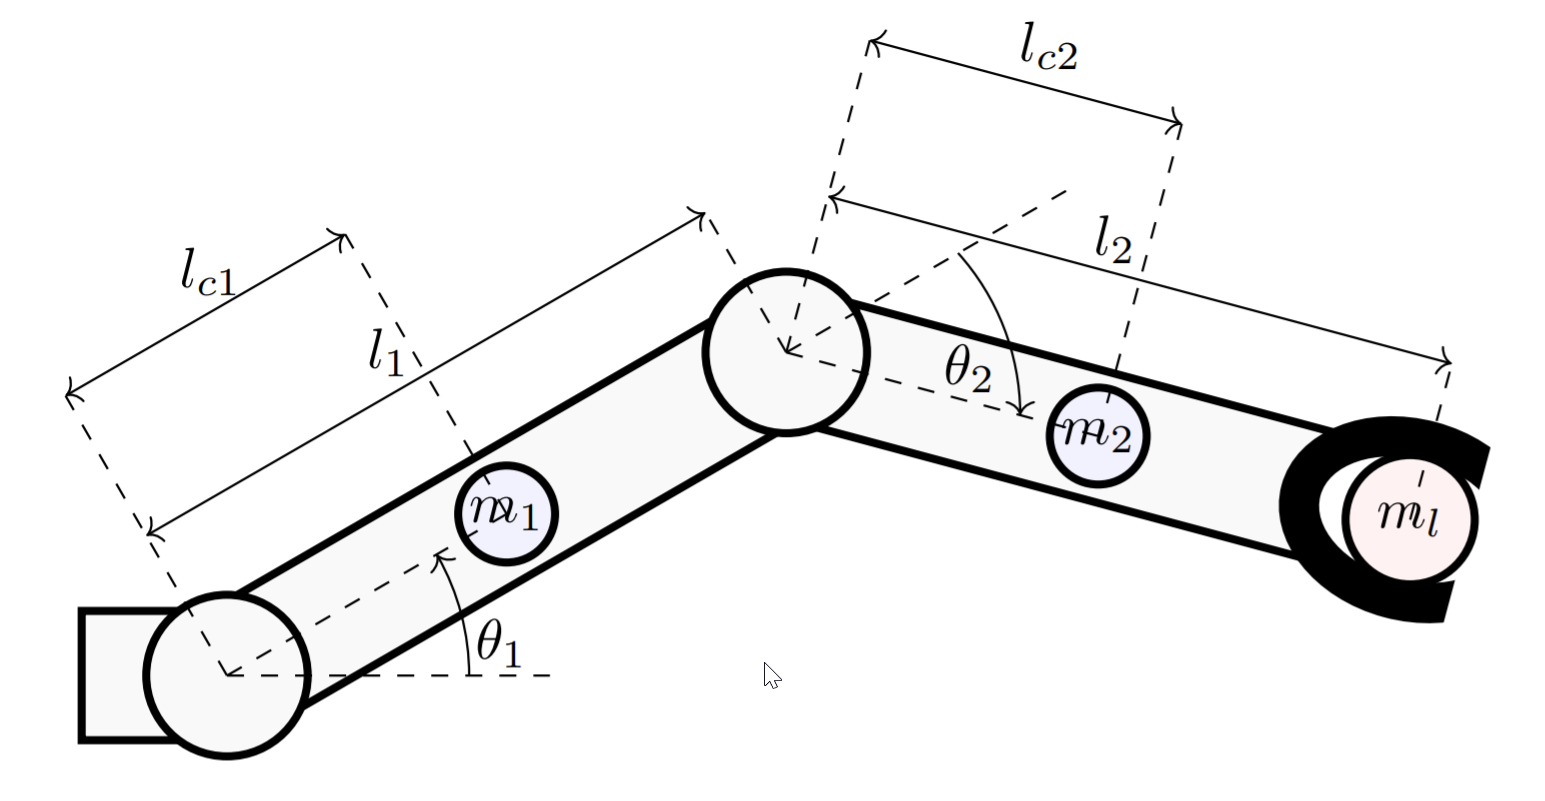
\includegraphics[width=14cm]{fig/fig1.png}
    \caption{Robotic arm system representation}
\end{figure}

\noindent\hspace{-2pt}
The angles $\theta_1$ and $\theta_2$ are the rotation angles of the two joints respectively, $l_1$ and $l_2$ are the 
lengths of the two parts of the arm and $m_1$, $m_2$ are the masses of the two parts gathered in the center of mass of 
each part respectively. The centers of mass are considered to be placed $l_{c1}$ and $l_{c2}$ after each joint. The arm 
holds a mass $m_l$, just as in figure 1. \\\\
If we assume 
$$
    \begin{cases}
        q_1 = \theta_1 \\ 
        q_2 = \theta_2
    \end{cases}
$$
so that 
\begin{align}
    q = [\theta_1 \; \theta_2]^T
\end{align}
the plant of the system will be 
\begin{align}
    H(q) \ddotq + C(q, \dotq) \dotq + g(q) = u
\end{align}
In the previous equation, $H$ is the $2 \times 2$, positive-definite and symmetric inertia matrix of the robotic arm: 
$$
    H(q) =  \begin{bmatrix}
            h_{11} & h_{12} \\
            h_{12} & h_{22}        
            \end{bmatrix}
$$
with 
$$h_{11} = m_{1} l_{c 1}^{2}+m_{2}\left(l_{c 2}^{2}+l_{1}^{2}+2 l_{1} l_{c 2} \cos q_{2}\right)+m_{l}\left(l_{2}^{2}+l_{1}^{2}+2 l_{1} l_{2} \cos q_{2}\right)+I_{1}+I_{2}$$
$$h_{12} = m_{2} l_{c 2}\left(l_{c 2}+l_{1} \cos q_{2}\right)+m_{l} l_{2}\left(l_{2}+l_{1} \cos q_{2}\right)+I_{2}$$
$$h_{22} = l_{c 2}^{2} m_{2}+l_{2}^{2} m_{l}+I_{2}$$
where $I_1$ and $I_2$ are the moments of inerita of each part respectively.
The matrix $C$ is defined as
$$C(q, \dotq) =     \begin{bmatrix}
                        -l_{1}\left(m_{2} l_{c 2}+m_{l} l_{2}\right) \sin q_{2} \dot{q}_{2} & -l_{1}\left(m_{2} l_{c 2}+m_{l} l_{2}\right) \sin q_{2}\left(\dot{q}_{2}+\dot{q}_{1}\right) \\
                        l_{1}\left(m_{2} l_{c 2}+m_{l} l_{2}\right) \sin q_{2} \dot{q}_{1} & 0
                    \end{bmatrix}
$$
and the vector $g$ as 
$$
    g(q) =  \begin{bmatrix}
                \left(m_{2} l_{c 2}+m_{l} l_{2}\right) g \cos \left(q_{1}+q_{2}\right)+\left(m_{2} l_{1}+m_{l} l_{1}+m_{1} l_{c 1}\right) g \cos q_{1} \\
                \left(m_{2} l_{c 2}+m_{l} l_{2}\right) g \cos \left(q_{1}+q_{2}\right)
            \end{bmatrix}
$$ \\

\noindent\hspace{-2pt}
The values of the known parameters of the system are presented in the following table:
\begin{table}[H]
    \centering
    \begin{tabular}{lllllll}
        \hline
        \textbf{parameter} & & & & & & \textbf{value}              \\ \hline
        $m_1$              & & & & & & $6 \, kg$                        \\
        $m_2$              & & & & & & $4 \, kg$                        \\
        $l_1$              & & & & & & $0.5 \, m$                       \\
        $l_2$              & & & & & & $0.4 \, m$                       \\
        $g$                & & & & & & $9.81 \, m/s^2$ \\ \hline
    \end{tabular}
    \caption{Values of known parameters}
\end{table}

\noindent\hspace{-2pt}
The following parameters are unknown, but we know their lower and upper bounds:
\begin{table}[H]
    \centering
    \begin{tabular}{llllll}
        \hline
        \textbf{parameter} & & \textbf{lower bound} & & \textbf{upper bound}              \\ \hline
        $l_{c1}$               & &  $0.1 \, m$ & &                 $0.4 \, m$                        \\
        $l_{c2}$               & &  $0.05 \, m$ & &                $0.3 \, m$                        \\
        $I_1$               & &     $0.02 \, kg \, m^2$ & &    $0.5 \, kg \, m^2$                       \\
        $I_2$               & &     $0.01 \, kg \, m^2$ & &    $0.15 \,kg \, m^2$                       \\
        $m_l$                  & &  $0 \, kg$ & &                  $2 \, kg$ \\ \hline
    \end{tabular}
    \caption{Bounds of unknown parameters}
\end{table}


\section{Controller design}
    The controller will be designed accoriding to \textit{sliding mode control} method. 
    Firstly we solve (2) for $\ddotq$:
    $$
        H \ddot{q}+C \dot{q}+g=u \Rightarrow 
    $$
    \begin{align}
        \ddot{q}=-H^{-1} \left( \mathrm{C} \dot{q} - g+ u \right)
    \end{align}
    Note that $H^{-1}$ exists and it is positive-definite, as $H$ is positive-definite. \\\\
    We also define the system state error 
    $$
        e = e(t) = q(t)-q_{d}(t) \; \in \R^{2 \times 1}
    $$
    where $q_d (t) \in \R^{2 \times 1}$ is the desired system state at a time moment $t$. In the \textit{regulation}
    process, $q_d$ will be constant, while in \textit{tracking} it will represent the desired signal to be tracked. 
    For our theoretical analysis, we considered the generic case, where $q_d$ is not constant (\textit{tracking}). 
    Note that in terms of convenience, we will represent all the signals of our system without their variable indicator.
    For example, $q(t)$ is represented as $q$ and $H(q)$ as $H$.
    \\\\
    We also have 
    $$
        \dot{e}=\dot{q}-\dot{q}_{d} \; \in \R^{2 \times 1}
    $$
    and
    $$
        \ddot{e}=\ddot{q}-\ddot{q}_{d} \; \in \R^{2 \times 1}
    $$
    Now, we define the \textit{sliding surface} 
    $$
        s = s(\dot{e}, e)=\dot{e}+\Lambda e = [0 \; \; 0]^T \;, \;\; \Lambda \in \R ^ {2\times2}\Rightarrow
    $$
    $$
        \dot{e}=-\Lambda e \Rightarrow 
    $$
    $$
        e \rightarrow 0 \;\; \text { for } \;\Lambda>0 
    $$
    So, if we force our system to the surface $s=0$, we guarantee that the system will tend to the desired behavior.
    We assume the \textit{Lyapunov} function canditate 
    $$
        V(s) = \frac{1}{2} s^T s = \frac{1}{2} \left[ s_1 \;\; s_2 \right] \left[ s_1 \;\; s_2 \right]^T = \frac{1}{2} s_1 ^2 + \frac{1}{2} s_2 ^2 \Rightarrow
    $$
    \begin{align}
        \dot{V}(s) = s_1 \dot{s_1} + s_2 \dot{s_2} = s^T \dot{s}        
    \end{align}
    We demand 
    $$
        \dot{V}(s) \le 0 \Leftrightarrow
    $$
    \begin{align}
        s^T \dot{s} \le 0       
    \end{align}
    with equality only for $s=0$. \\\\
    We just have to design a control input $u$, so that the system satisfies (5). \\\\
    We have 
    $$  
        \dot{s}=\ddot{e}+\Lambda \dot{e}=\ddot{q}-\ddot{q}_{d}+\Lambda \dot{e} \Rightarrow 
    $$
    \begin{align}
        \dot{s} = -H^{-1}(C \dot{q}+g-u)-\ddot{q} d+\Lambda \dot{e}
    \end{align}
    and we define the equivalent input $u_{eq}$ for $\dot{s} = 0$, so from (6) we get
    $$
        u_{e q}=C \dot{q}+g+H \ddot{q}_{d}-H \Lambda \dot{e}
    $$
    and we use some parameter estimations in the bounds of table 2 for the unknown parameters 
    of $u_{eq}$, so we have 
    $$
        \hat{u}_{e q}=\hat{C} \dot{q}+\hat{g}+\hat{H} \ddot{q}_{d}-\hat{H} \Lambda \dot{e}
    $$
    In order to reduce chattering, we will use $\hat{u_{eq}}$ in our controller.
    So, accoriding to \textit{sliding mode control}, the control input will be 
    \begin{align}
        u=\hat{u}_{e q}- \rho \odot [\operatorname{sat}(s_1, \varepsilon) \; \operatorname{sat}(s_2, \varepsilon)]^T
    \end{align}
    where $\rho$ $\in \R^{2\times1}$ will be defined later and
    $$
        \operatorname{sat}(x)=\left\{\begin{array}{c}
        x / \varepsilon \, ,\quad \left| x \right| \leq \varepsilon \\
        1 \, , \quad x > \varepsilon \\
        -1 \, , \quad x < -\varepsilon
        \end{array}\right.
    $$
    \\
    Replacing (7) in (2) we get
    $$
        H \ddot{q} + C \dot{q} + g = 
        \hat{C} \dot{q} + \hat{g} + \hat{H} \ddot{q}_{d} - \hat{H} \Lambda \dot{e} - \rho \odot [\operatorname{sat}(s_1, \varepsilon) \; \operatorname{sat}(s_2, \varepsilon)]^T \Rightarrow
    $$
    $$
        H \ddot{q}=\hat{C} \dot{q} + \hat{g} + \hat{H} \ddot{q}_{d} -\hat{H} \Lambda \dot{e} - 
        \rho \odot [\operatorname{sat}(s_1, \varepsilon) \; \operatorname{sat}(s_2, \varepsilon)]^T - C \dot{q} - g \Rightarrow
    $$
    $$
        H \ddot{q} - H \ddot{q}_{d} + H \Lambda \dot{e} = 
        (\hat{H}-H) \ddot{q}_{d} + (\hat{C}-C) \dot{q} + (\hat{g}-g)- (\hat{H}-H) \Lambda \dot{e}- \rho \odot [\operatorname{sat}(s_1, \varepsilon) \; \operatorname{sat}(s_2, \varepsilon)]^T \Rightarrow
    $$
    $$
        H (\ddot{q} - \ddot{q}_{d} + \Lambda \dot{e}) = 
        \tilde{H} (\ddot{q}_{d} - \Lambda \dot{e}) + \tilde{C} \dot{q} + \tilde{g} - \rho \odot [\operatorname{sat}(s_1, \varepsilon) \; \operatorname{sat}(s_2, \varepsilon)]^T \Rightarrow
    $$
    \begin{align}
        H \dot{s} = 
        \tilde{H} (\ddot{q}_{d} - \Lambda \dot{e}) + \tilde{C} \dot{q} + \tilde{g} - \rho \odot [\operatorname{sat}(s_1, \varepsilon) \; \operatorname{sat}(s_2, \varepsilon)]^T
    \end{align}
    where 
    $$
    \begin{cases}
        \tilde{H} = \hat{H} - H \\ 
        \tilde{C} = \hat{C} - C \\ 
        \tilde{g} = \hat{g} - g 
    \end{cases}
    $$
    are the error matrices between the estimations 
    of system matrices and the real system matrices. 
    From (8), multiplying the two parts of the equiation by left with $H^{-1}$ and subsequently multiplying by left with $s^T$, 
    we get 
    $$
        s^T \dot{s} = 
        s^T H^{-1} \left[ \tilde{H} (\ddot{q}_{d} - 
        \Lambda \dot{e}) + \tilde{C} \dot{q} + \tilde{g} - 
        \rho \odot [\operatorname{sat}(s_1, \varepsilon) \; \operatorname{sat}(s_2, \varepsilon)]^T \right]
    $$
    We select
    \begin{align}
        \rho = \tilde{H}_{max} | \ddot{q}_{d} - 
        \Lambda \dot{e} | + \tilde{C}_{max} | \dot{q} | + \tilde{g}_{max} + [c \;\; c]^T        
    \end{align}
    where $\tilde{H}_{max}$, $\tilde{C}_{max}$ and $\tilde{g}_{max}$ are the system matrices with maximum 
    values in all of their elements and $|v| = [|v_1| \;\; |v_2|]^T$ for a vector $v \in \R^2$. 
    The maximum values of the elements of the matrices occur for the maximum values of the unknown parameter errors: 
    $$
        \begin{cases}
            \tilde{l_{c1}}_{max} = 0.3 \\
            \tilde{l_{c2}}_{max} = 0.25 \\
            \tilde{I_{1}}_{max} = 0.48 \\
            \tilde{I_{2}}_{max} = 0.14 \\
            \tilde{l_{m_l}}_{max} = 2 \\
        \end{cases}
    $$
    according to table 2, as it can be proved that they are increasing with repsect to those errors. Replacing (9) in (8) 
    we can reach the inequality 
    \begin{align}
        s^T \dot{s} \le - \, |s^T| \, |H^{-1}| \, [c \;\; c]^T \;, \;\; c>0
    \end{align}
    $$
        \Rightarrow s^T \dot{s} \le 0       
    $$
    with equality only for $s=0$, so the desired condition (5) is satisfied and $s \rightarrow 0$. Thus, the system 
    slides through $s=0$ surface and $q \rightarrow q_d$. The control goal has been achieved.

\section{Simulation}
The system simulated in \textit{MALTAB} with initial conditions 
$$
    \begin{cases}
        q_0 = [\frac{\pi}{3} \;\; \frac{\pi}{3}]^T \\
        \dot{q}_0 = [0 \;\; 0]^T
    \end{cases}
$$
\\
For the real system plant the following values of the unknown parameters were used:
\begin{table}[H]
    \centering
    \begin{tabular}{lllllll}
        \hline
        \textbf{parameter} & & & & & & \textbf{value}              \\ \hline
        $l_{c1}$              & & & & & & $0.2 \, m$                        \\
        $l_{c2}$              & & & & & & $0.1 \, m$                        \\
        $I_1$              & & & & & & $0.43 \, kg \, m^2$                       \\
        $I_2$              & & & & & & $0.05 \, kg \, m^2$                       \\
        $m_l$                & & & & & & $0.5 \, kg$ \\ \hline
    \end{tabular}
    \caption{Real values of unknown parameters}
\end{table}

\noindent\hspace{-2pt}
Note that the values of table 3 are considered as unknown, so they were not used in the controller implementation.
They were only used to simulate the behavior of the real system. The system was simulated in two different cases: 
\textbf{regulation}, where the control goal was to make the system state vector $q$ to converge to a desired constant 
state vector $q_d$, as $t\rightarrow \infty$ and \textbf{tracking}, where the control goal was to to make the system state vector $q$ to 
track a reference signal $q_d(t)$, as $t \rightarrow \infty$.

\subsection{Regulation}
In the first case, we assume 
$$
    \begin{cases}
        q_d = \big[ \frac{\pi}{2} \;\;\; -\frac{\pi}{3} \big]^T \\
        \dot{q_d} = [0 \;\; 0]^T \\
        \ddot{q_d} = [0 \;\; 0]^T
    \end{cases}
$$
and we set these values in the control input $u$. The parameter $\varepsilon$ of the \textit{saturation} function was 
set equal to the value $0.05$, which provided satisfying results. The further analysis of this parameter is out of scope 
of this project. Also, we select $c = 0.5$. The effect of this parameter will be discussed later.
The selection of matrix $\Lambda$ of the \textit{sliding surface} was crucial for the system behavior. 
After tuning, the selected matrix was 
$$
    \Lambda = \begin{bmatrix}
        5 & 0 \\
        0 & 5
    \end{bmatrix}
$$
We will present the system behavior through some diagrams for the selected parameters $c$ and $\Lambda$ and then we will compare 
the results with some other values of the parameters.
\subsubsection{Results for the selected parameters}
\begin{figure}[H]
    \centering
    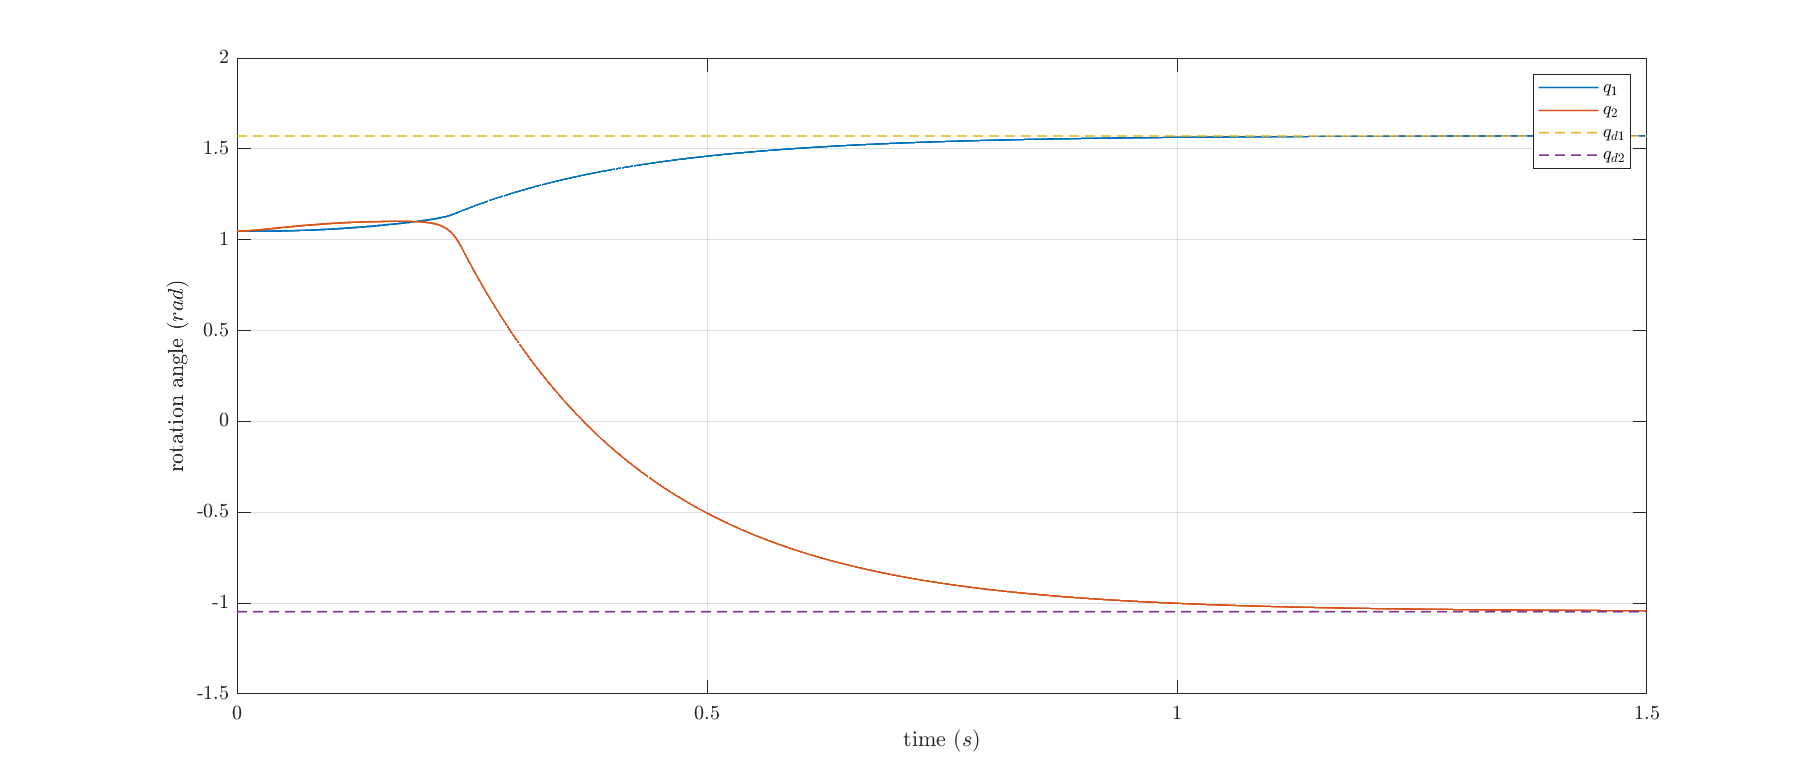
\includegraphics[width=15cm]{fig/sim1/q.png}
    \caption{Rotation angles with respect to time}
\end{figure}
\vspace*{-0.5cm}
\begin{figure}[H]
    \centering
    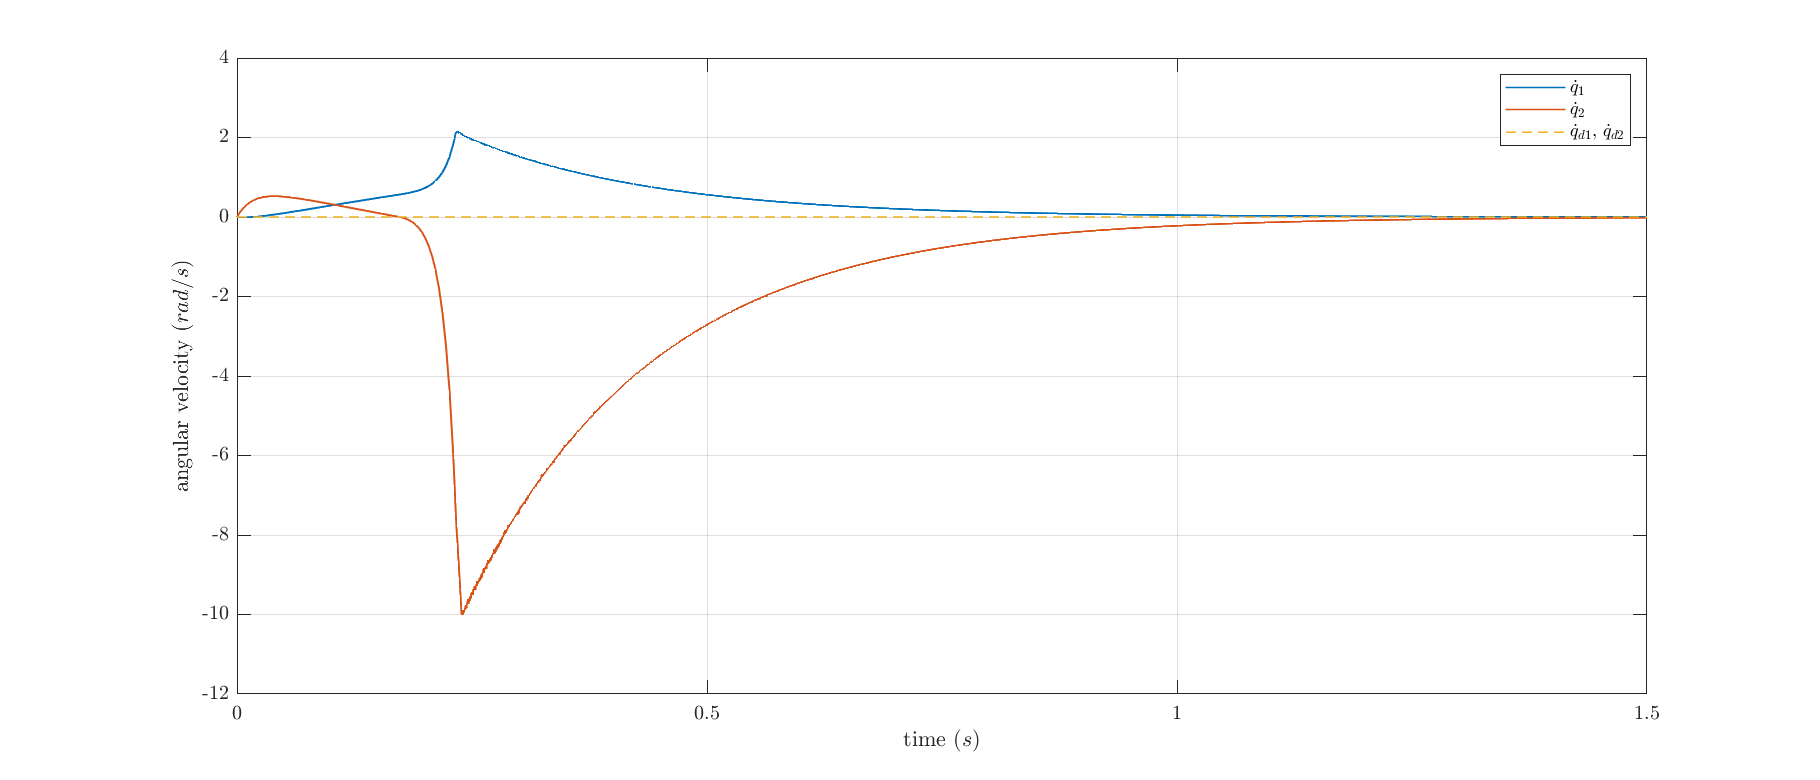
\includegraphics[width=15cm]{fig/sim1/qdot.png}
    \caption{Angular velocities with respect to time}
\end{figure}
\begin{figure}[H]
    \centering
    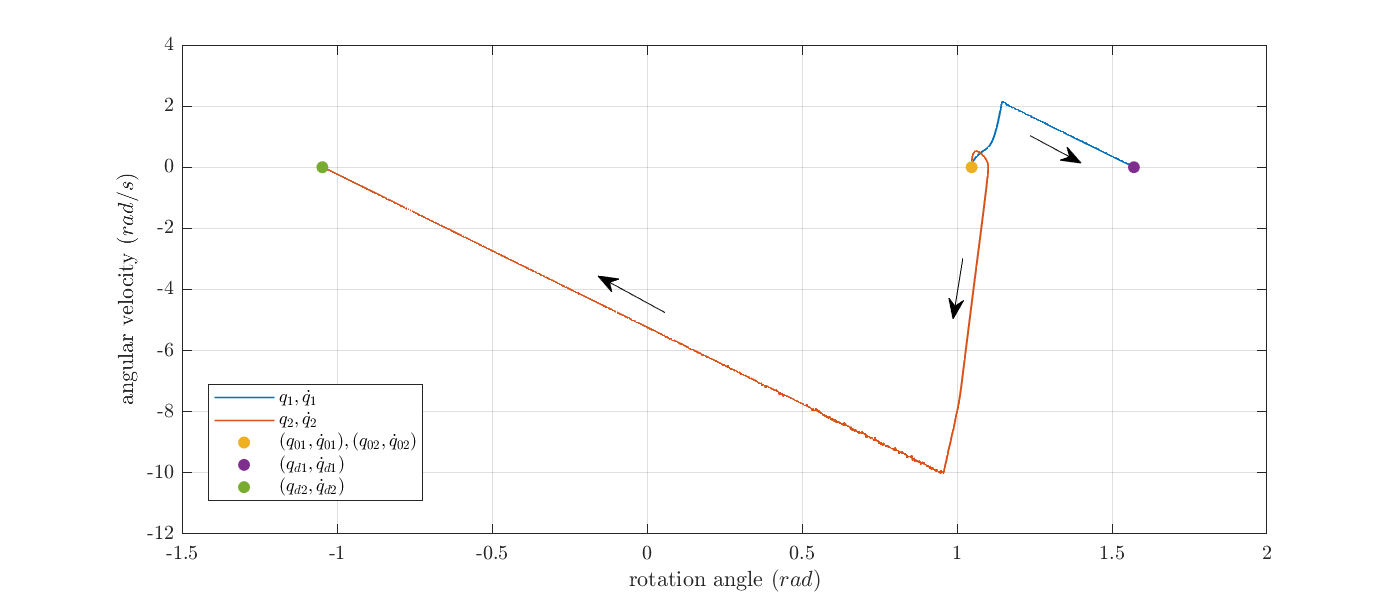
\includegraphics[width=15cm]{fig/sim1/phaseplane.png}
    \caption{Phase plane of system states}
\end{figure}
\begin{figure}[H]
    \centering
    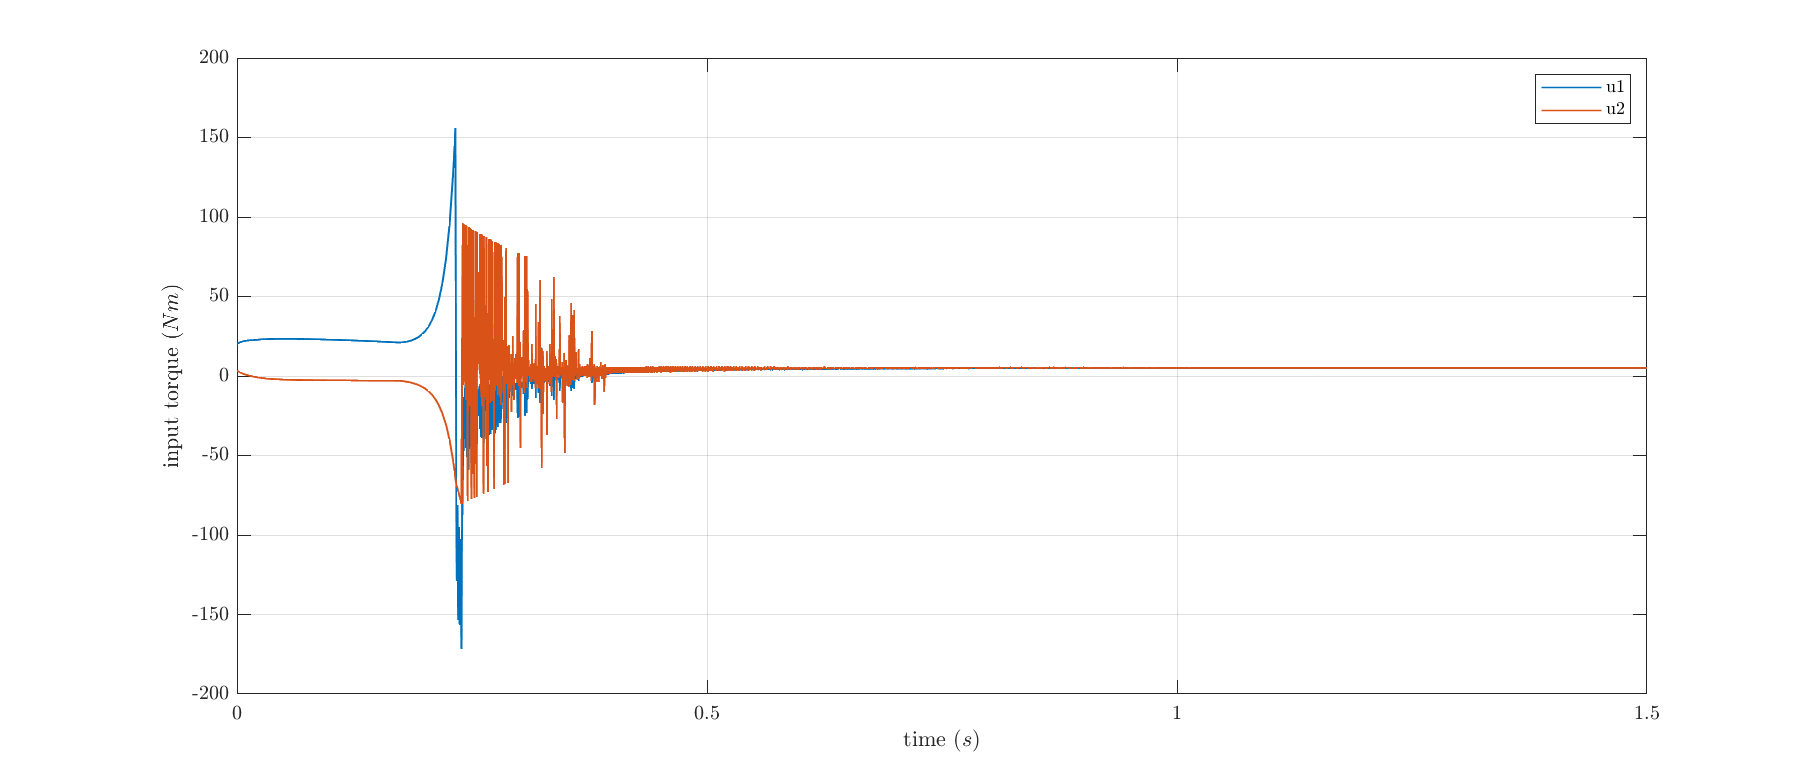
\includegraphics[width=15cm]{fig/sim1/u.png}
    \caption{Control input with respect to time}
\end{figure}
\begin{figure}[H]
    \centering
    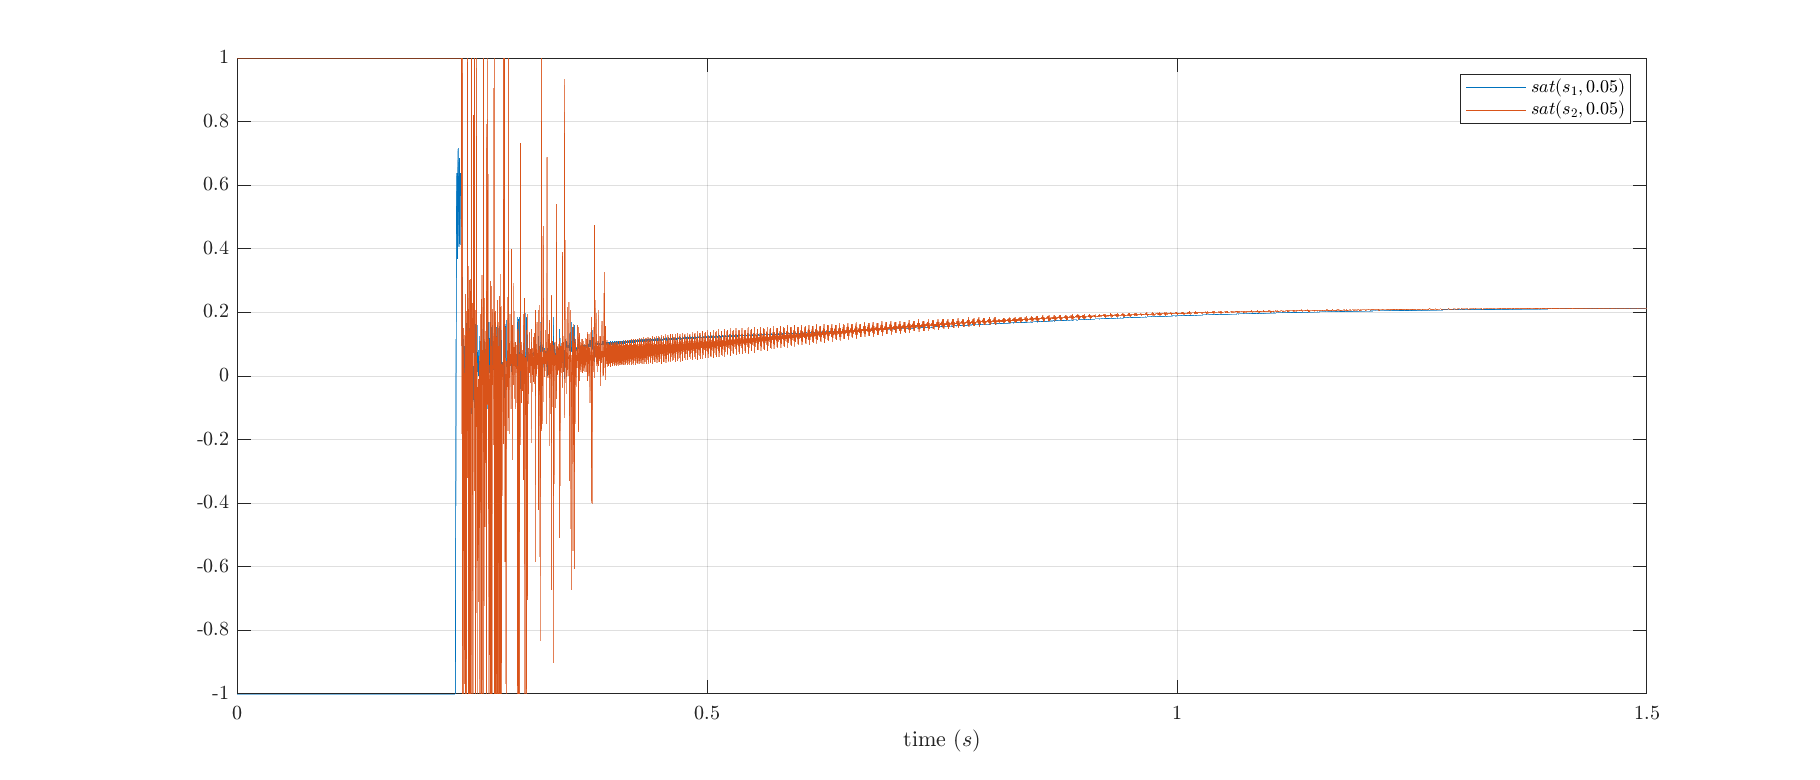
\includegraphics[width=15cm]{fig/sim1/sat.png}
    \caption{Saturation function of controller with respect to time}
\end{figure}
\begin{figure}[H]
    \centering
    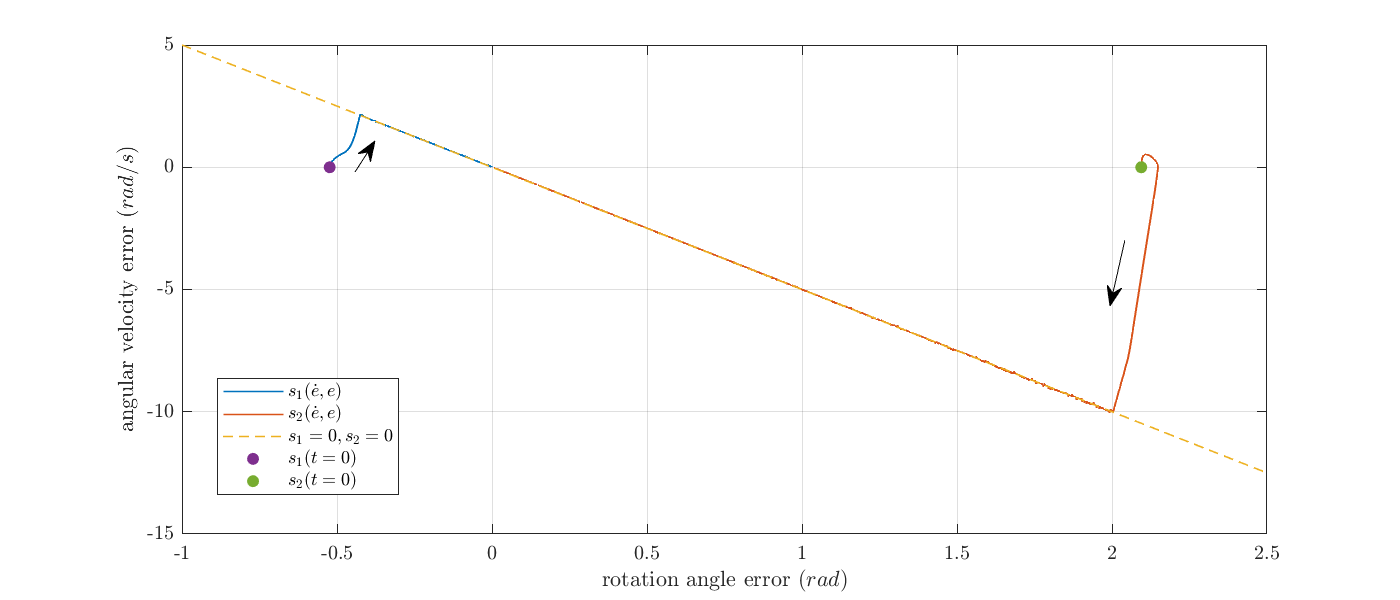
\includegraphics[width=15cm]{fig/sim1/sliding.png}
    \caption{Convergence to sliding surface}
\end{figure}
\begin{figure}[H]
    \centering
    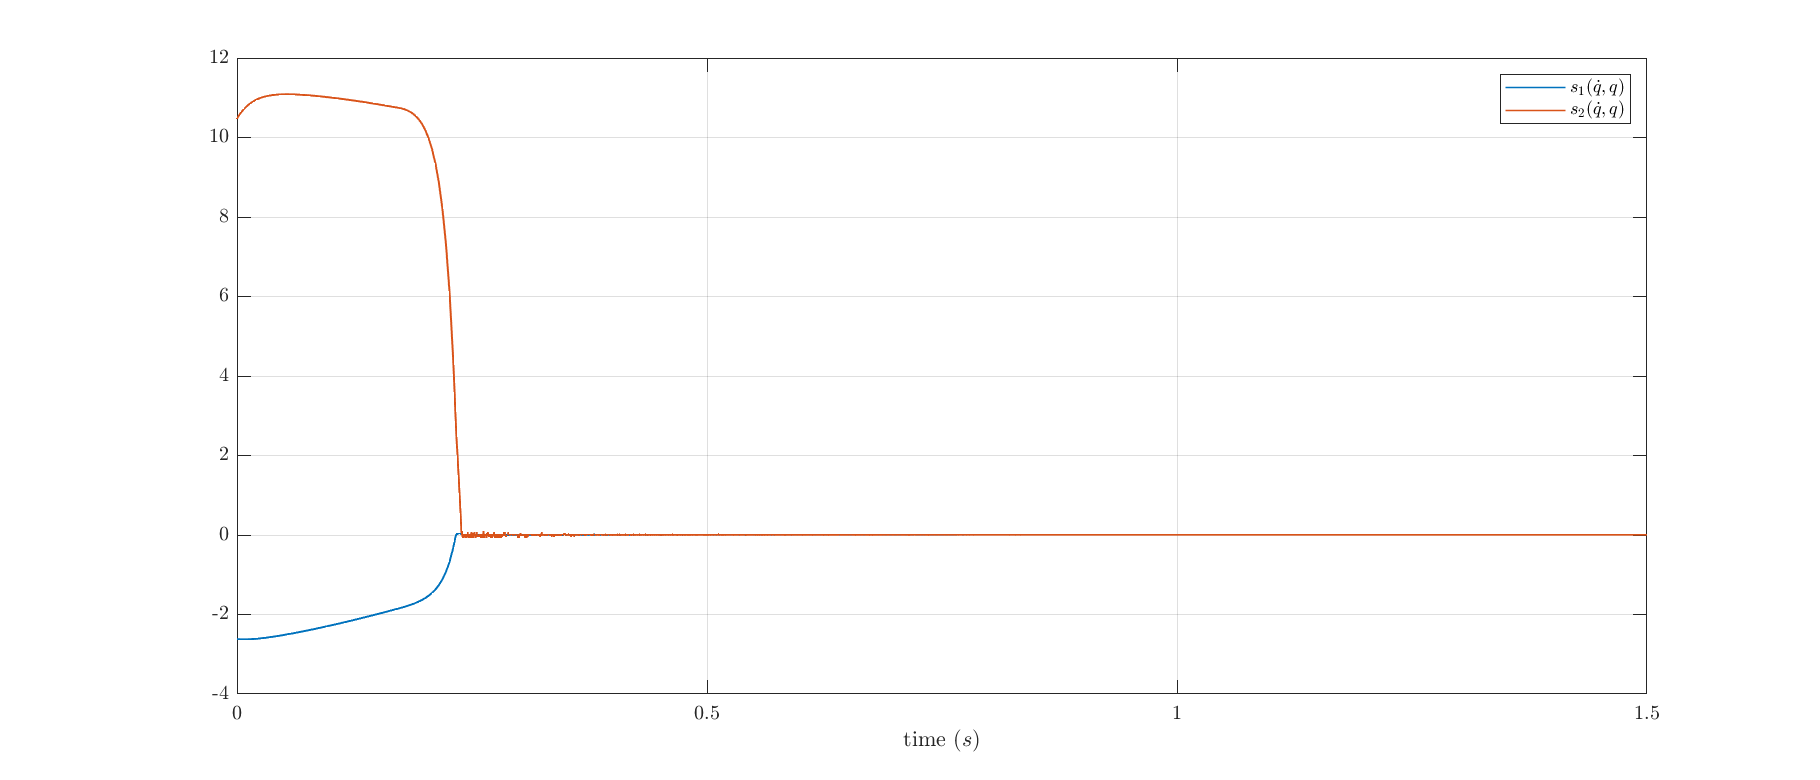
\includegraphics[width=15cm]{fig/sim1/s.png}
    \caption{Surface $s(\dot{q}, q)$ with respect to time}
\end{figure}
\begin{figure}[H]
    \centering
    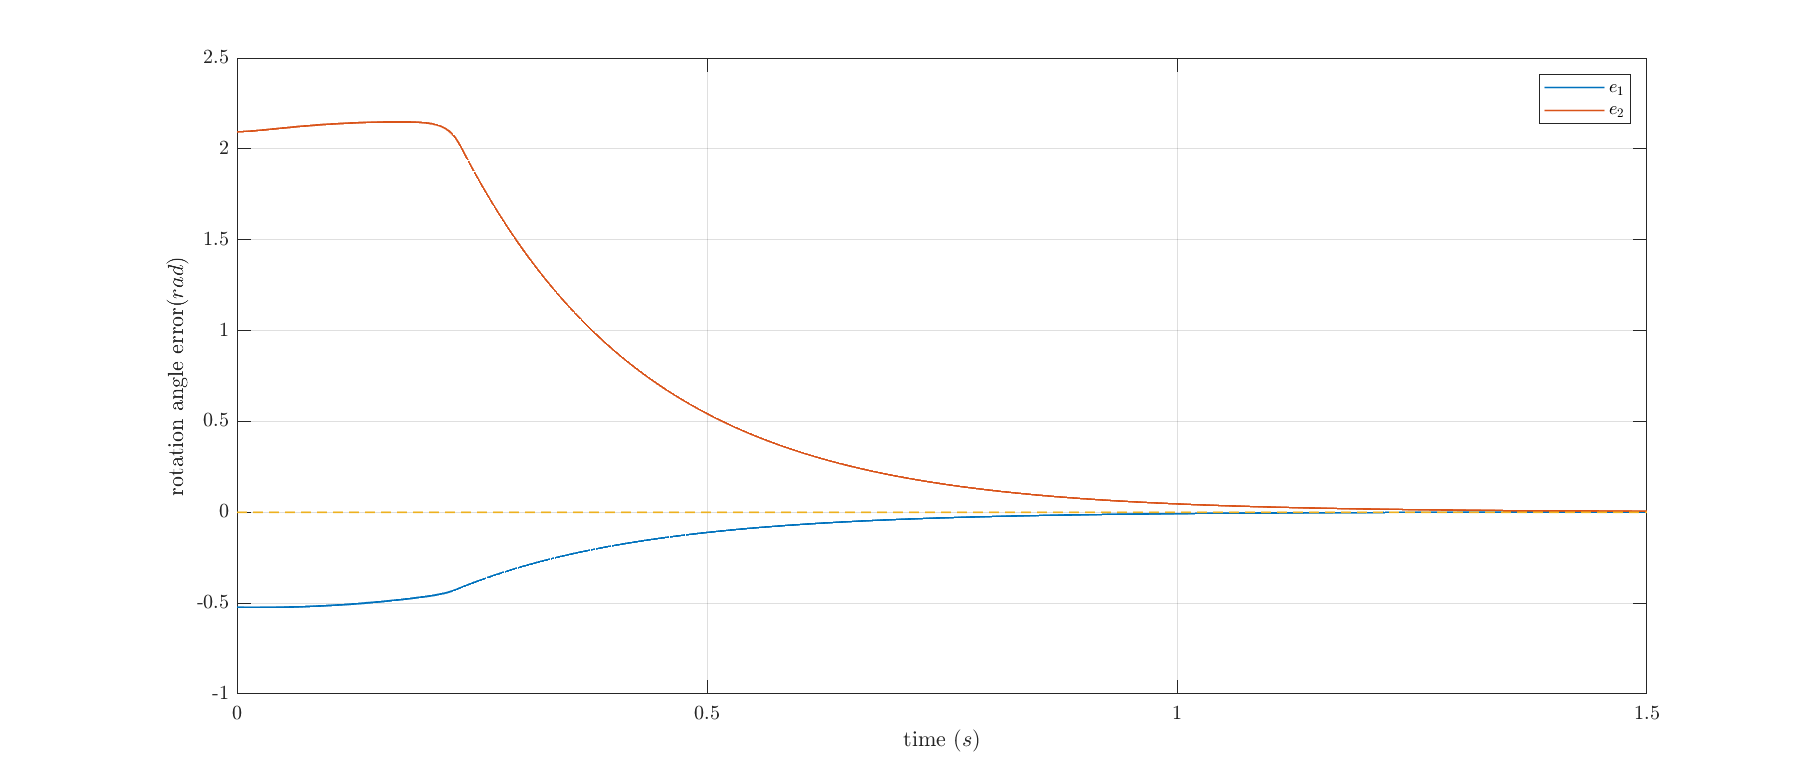
\includegraphics[width=15cm]{fig/sim1/e.png}
    \caption{State error with respect to time}
\end{figure}

\noindent\hspace{-2pt}
\begin{itemize}
    \item In figure 2, we can see that the system rotation angles converge to the desired values fast enough without undesirable behavior (overshot, oscillation, etc).
    \item In figure 3, we notice that the angular velocities converge to the desired values too. 
    \item In figure 5, we can see the discontinuities in the control input due to saturation function (figure 6). These discontinuities disappear when $s$ gets into 
    the $|\varepsilon|$ bounds and the control input becomes more stable, tending to a constant value while $t \rightarrow \infty$. 
    \item All the signals of the system are bounded (figures 1,2, 5).
    \item The theoretical \textit{rise times} for $s_1$ and $s_2$ are 
    $$  \begin{cases}
            t_{r1} \le \frac{|s_1(0)|}{c} = \frac{2.618}{0.5} = 5.236 s\\
            t_{r2} \le \frac{|s_2(0)|}{c} = \frac{10.472}{0.5} = 20.944 s
        \end{cases} 
    $$
    which is clearly validated by figure 8, as we see that $s(\dot{q}, q)$ reaches $s=0$ much faster.
    \item In figure 5 we can see the \textit{phase plane} of the system states as they converge to the equilibrium point.
    \item In figure 7 the convergence of the system to the \textit{sliding surface} is visible. In figure 8 we can see the time 
    when the system reaches the \textit{sliding surface}. Since that time (about 0.25 seconds), the state errors start converging 
    to zero, validating our theoretical expectations, as the error slides through the surface $s=0$.
    \item Moreover, by the time the system reaches the \textit{sliding surface}, the power of the input torque (figure 5) starts 
    becoming stable.
\end{itemize}

\subsubsection{Parameter $c$ analysis}
From (10) we can export that the increase of parameter $c$ can make the \textit{Lyapunov} derivative more negative, so the system 
will reach faster $s=0$ state. We provide an example for $c=10$ (larger than the selected $c=0.5$) and $\Lambda$ equal to the selected:
\begin{figure}[H]
    \centering
    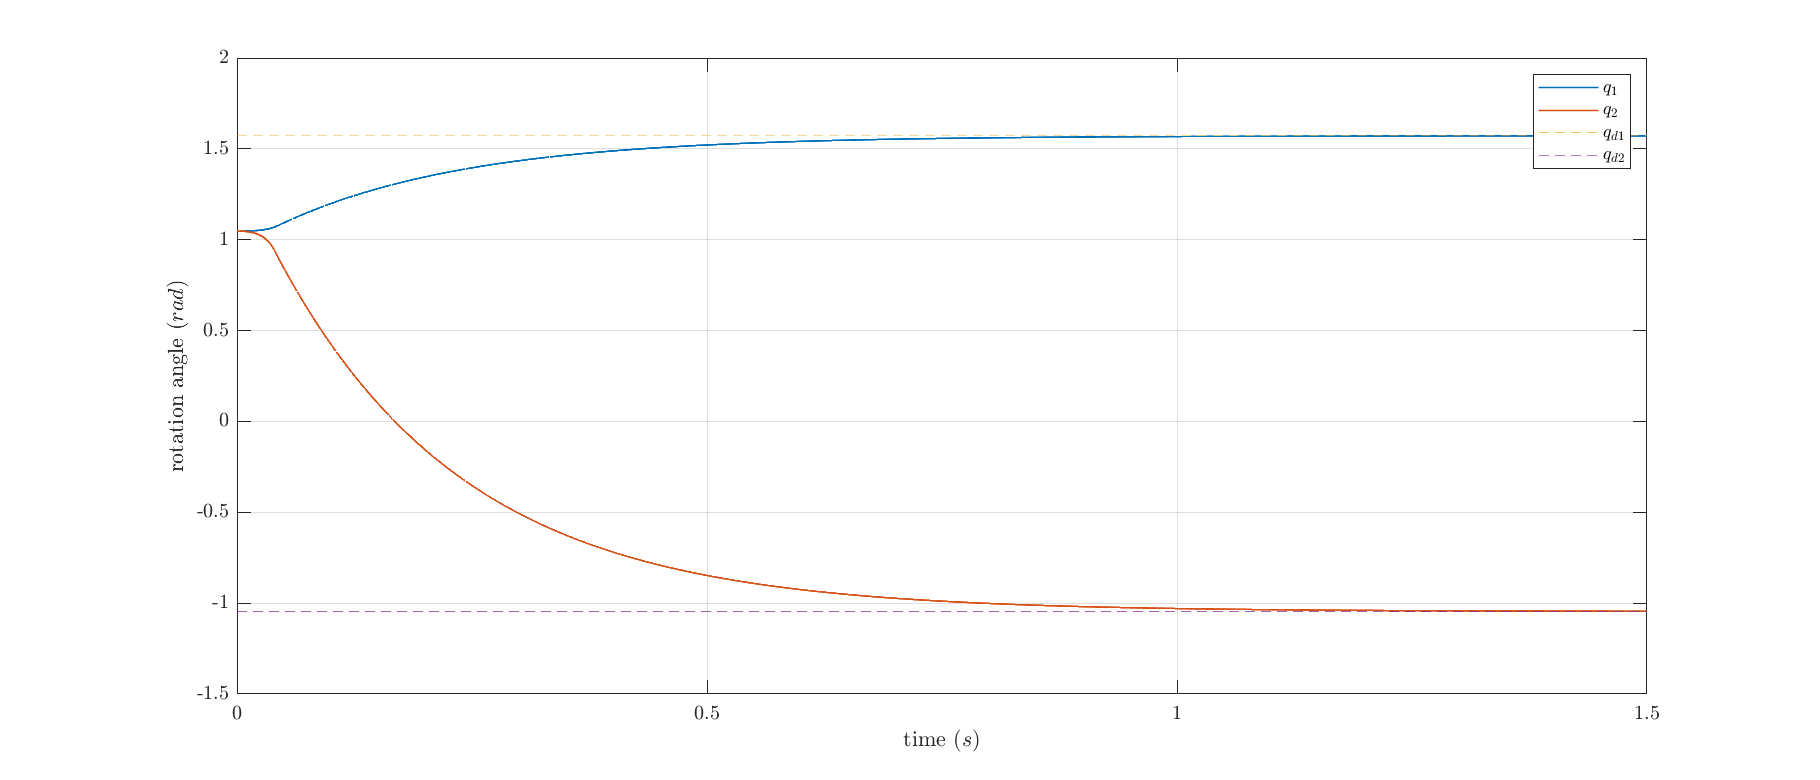
\includegraphics[width=15cm]{fig/sim1/qc10.png}
    \caption{Rotation angles with respect to time for $c=10$}
\end{figure}
\begin{figure}[H]
    \centering
    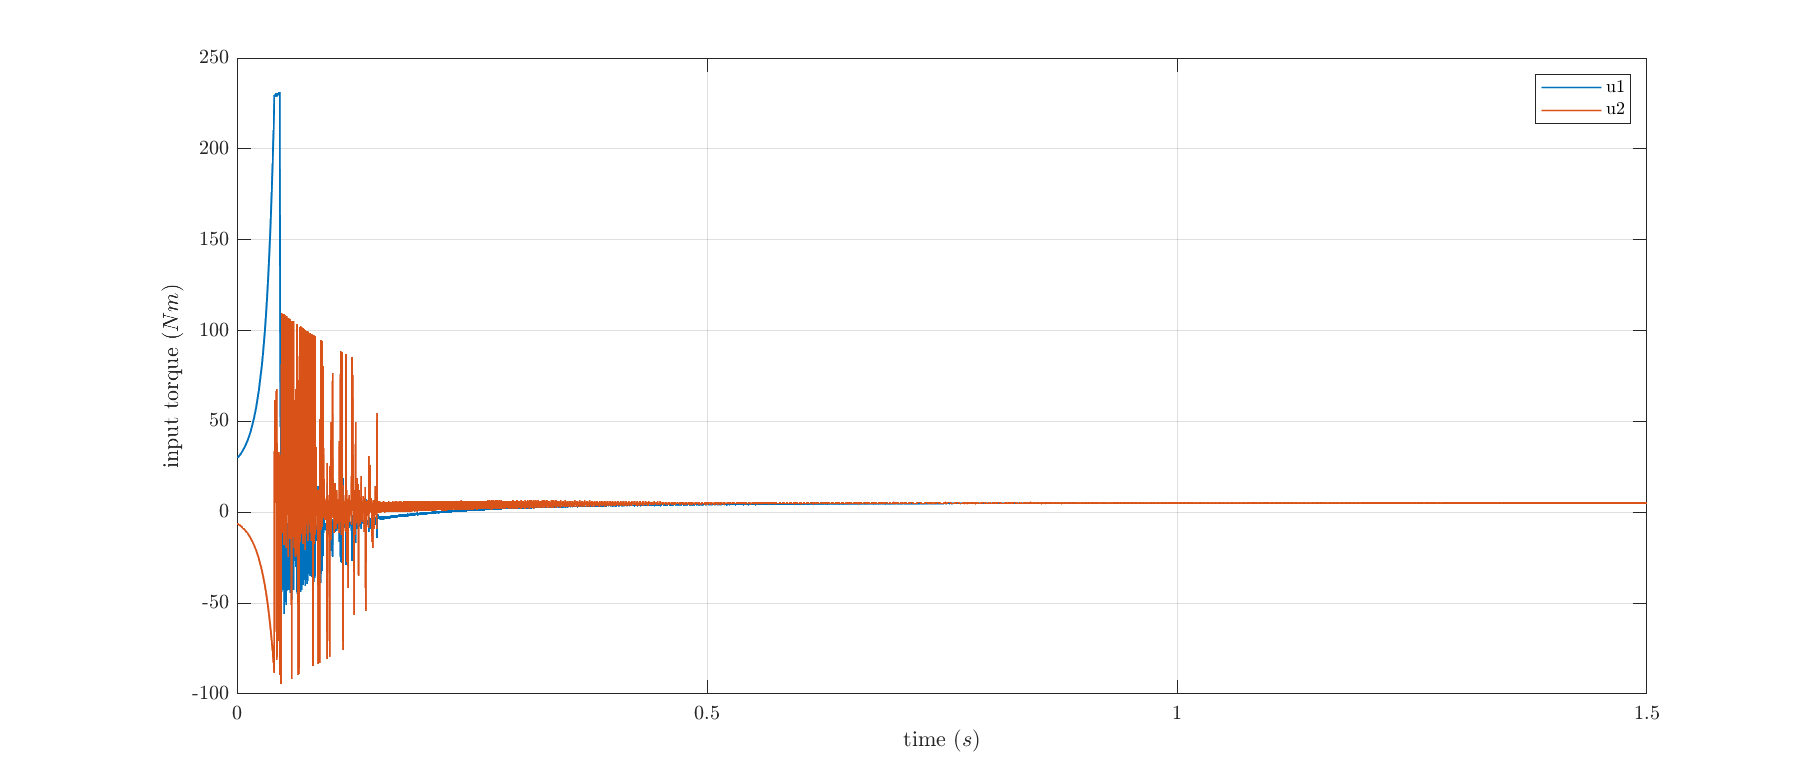
\includegraphics[width=15cm]{fig/sim1/uc10.png}
    \caption{Control input with respect to time for $c=10$}
\end{figure}
\begin{figure}[H]
    \centering
    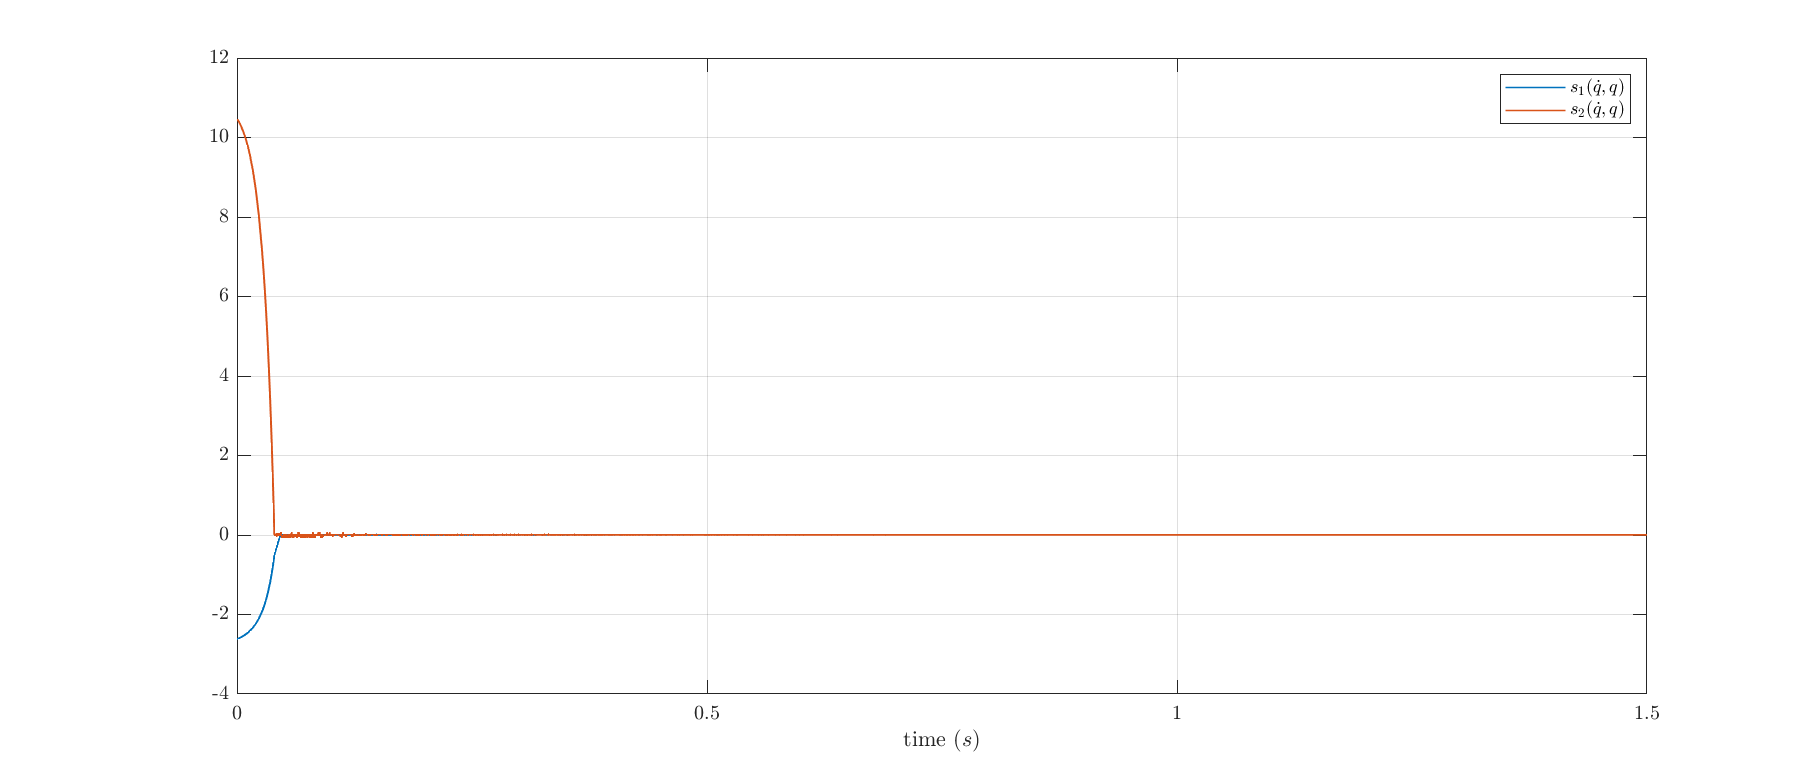
\includegraphics[width=15cm]{fig/sim1/sc10.png}
    \caption{Surface $s(\dot{q}, q)$ with respect to time for $c=10$}
\end{figure}
\begin{figure}[H]
    \centering
    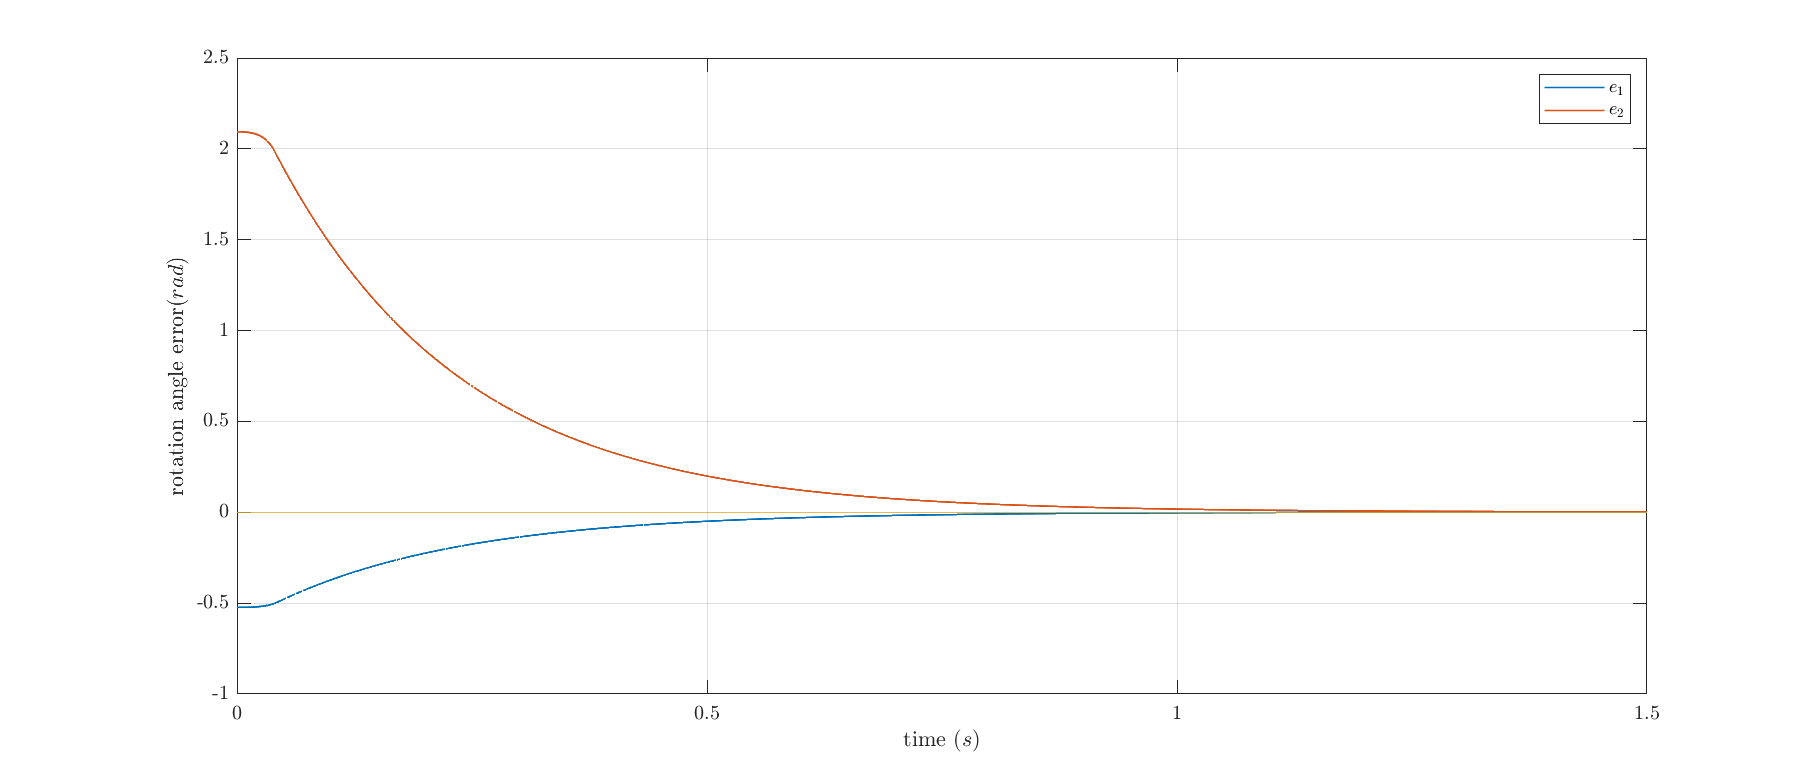
\includegraphics[width=15cm]{fig/sim1/ec10.png}
    \caption{State error with respect to time for $c=10$}
\end{figure}

\noindent\hspace{-2pt}
Comparing figures 8 and 12, our theoretical approach is validated, as $s(\dot{q}, q)$ converges much faster to zero 
for the increased value of $c$. However, comparing figures 2 and 10 we see that the improvement in system state convergence time 
is not important, as parameter $c$ affect the system speed until it reaches $s=0$ surface. Since then, the convergence speed is 
defined by some parameters that will be analyzed in the next subsection. Overall, increase of parameter $c$ only achieves to 
reduce the time until the state error starts decreasing (figure 13 ) and increases the maximum amplitude of control signal (figure 11). 
As a result, it was prefered to keep the parameter at the value $c=0.5$.

\subsubsection{Parameter matrix $\Lambda$ analysis}
Now, we will examine some other candidate matrices $\Lambda$ with constant $c=0.5$. We assume 
$$
    \Lambda =   \begin{bmatrix}
                    \lambda_1 & 0 \\
                    0 & \lambda_2
                \end{bmatrix}
$$
In the previous results, we selected $\lambda_1 = \lambda_2 = 5$. From the definition of the \textit{sliding surface} we get 
$$
    \dot{e} = - \Lambda e \Rightarrow
$$
$$
    \begin{cases} \dot{e}_1 = - \lambda_1 e_1 \\ \dot{e}_2 = - \lambda_2 e_2 \end{cases}
$$
so it is obvious that $\lambda_1$ and $\lambda_2$ determine the speed of the error convergence to zero, 
after the system reaches the \textit{sliding surface}. For $\lambda_1 = \lambda_2 = 0.5$ we present the following diagram:
\begin{figure}[H]
    \centering
    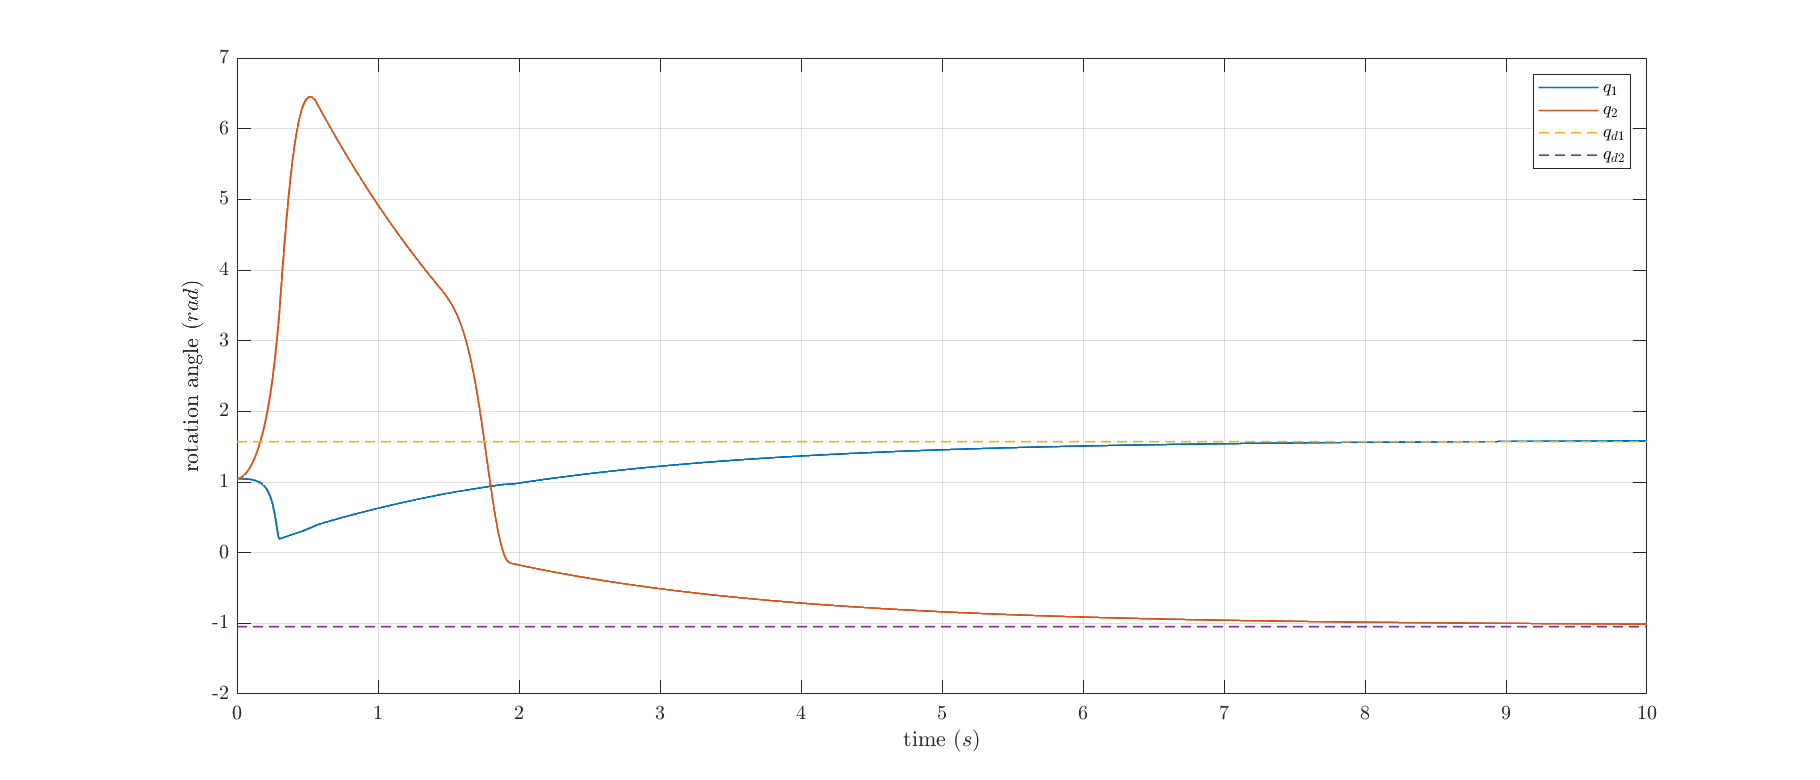
\includegraphics[width=15cm]{fig/sim1/q05.png}
    \caption{Rotation angles with respect to time for $\lambda_1 = \lambda_2 = 0.5$}
\end{figure}

\noindent\hspace{-2pt}
We can notice that the convergence is much slower in comparison with figure 2 ($\lambda_1 = \lambda_2 = 5$), as expected. Also, $q_2$ presents 
high overshot. We conclude that these values of parameters lead to undesirable behavior of the system. \\\\
Now we set $\lambda_1 = \lambda_2 = 25$ and we expect faster convergence:
\begin{figure}[H]
    \centering
    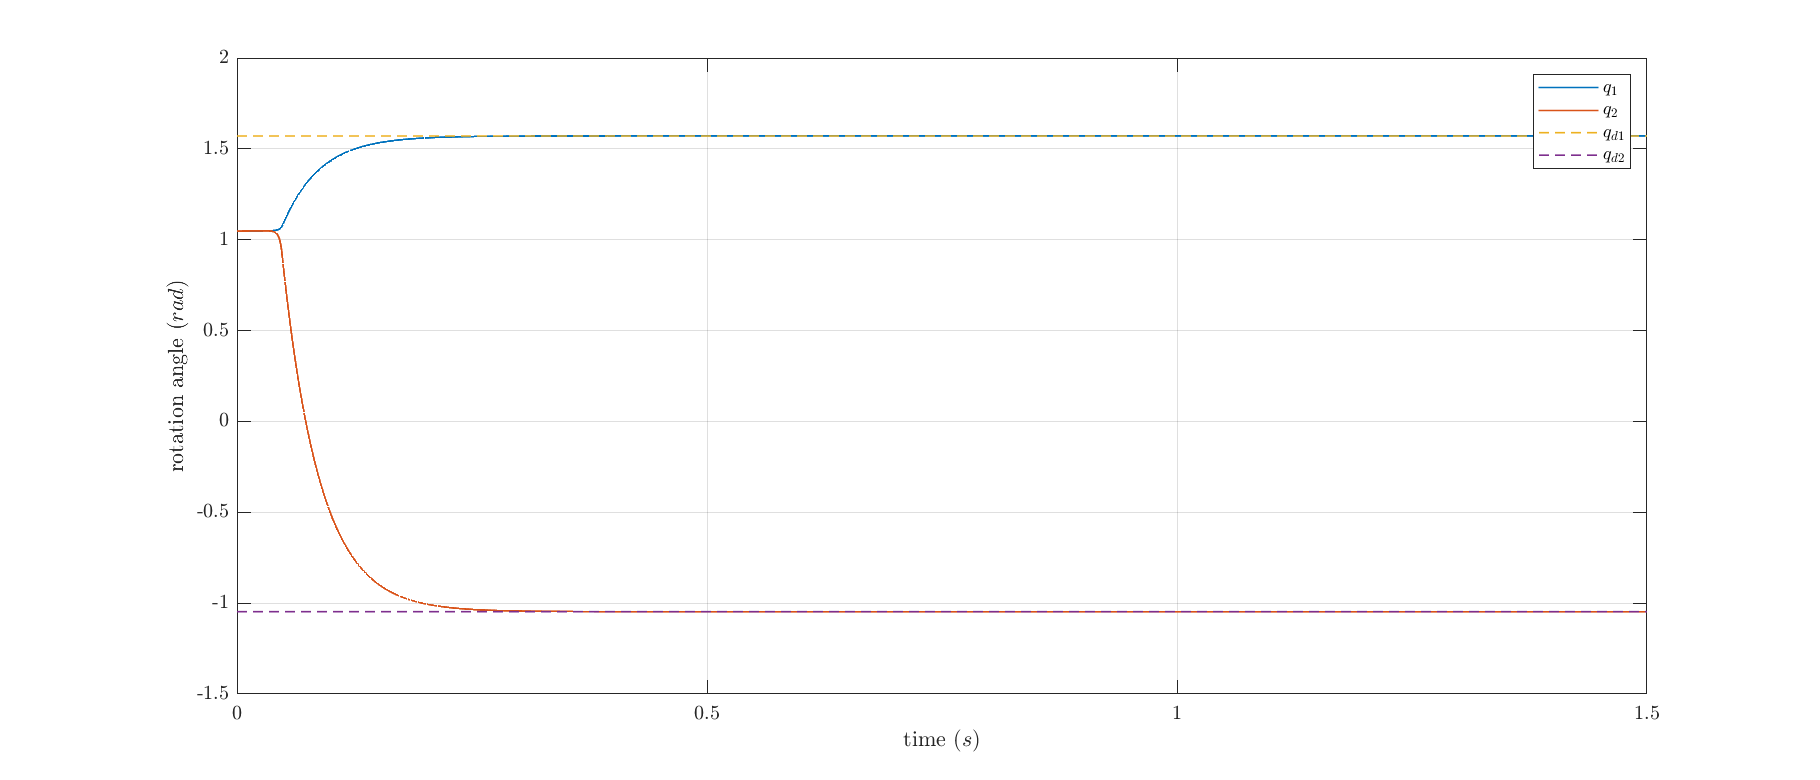
\includegraphics[width=15cm]{fig/sim1/q25.png}
    \caption{Rotation angles with respect to time for $\lambda_1 = \lambda_2 = 25$}
\end{figure}

\newpage
\noindent\hspace{-2pt}
Actually our prediction is confirmed and the convergence is even faster than figure 2. However, if we look at the control input: 
\begin{figure}[H]
    \centering
    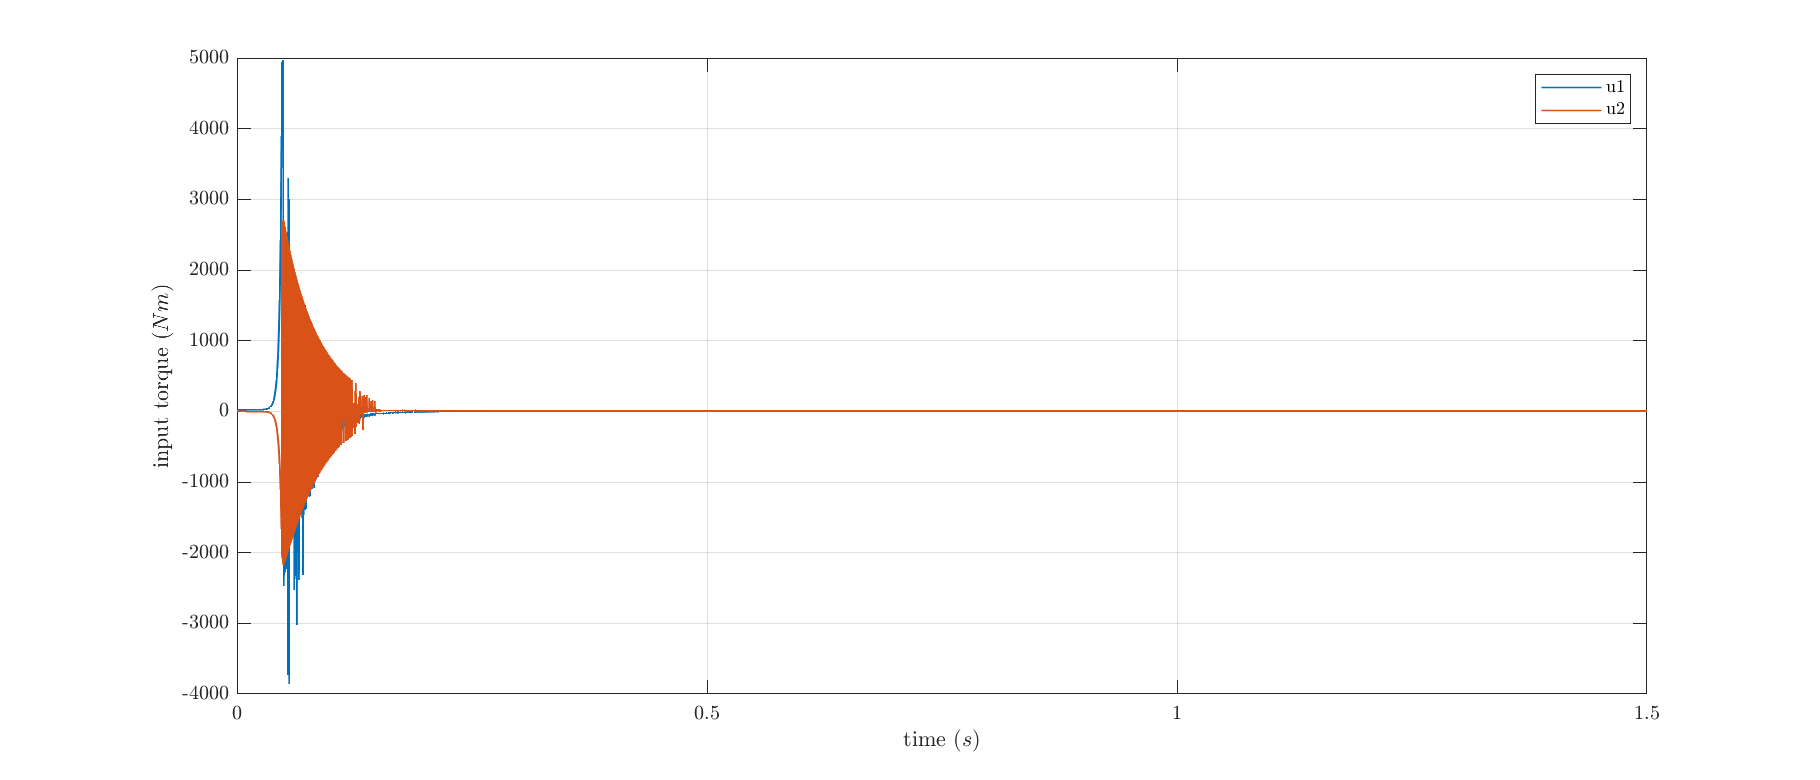
\includegraphics[width=15cm]{fig/sim1/u25.png}
    \caption{Control input with respect to time for $\lambda_1 = \lambda_2 = 25$}
\end{figure}

\noindent\hspace{-2pt}
we can see that it takes much larger values compared to figure 5, until the system reaches the \textit{sliding surface}. This is often 
unwanted, as the controller demands huge amount of power leading to problems like high energy consumption, costruction cost, etc.
Taken into account criteria like these, we tuned the system with respect to parameters $\lambda_1$ and $ \lambda_2$ and selected 
$\lambda_1 = \lambda_2 = 5$.

\subsection{Tracking}
Now we assume the desired state orbit
$$
    q_d = \begin{bmatrix}
        \frac{\pi}{4} + \frac{\pi}{6} \sin (0.2 \pi t)\\
        -\frac{\pi}{3} + \frac{\pi}{3} \cos (0.2 \pi t)
    \end{bmatrix}
$$
The control goal is to make the state vector $q$ to track the orbit $q_d$ as $t \rightarrow \infty$, 
using \textit{sliding mode control}. As previously, we set in (7) the new desired state vector $q_d$ 
and we have to select the parameters $c$ and $\Lambda$ of the control input. After tuning, we selected 
$c=10$, $\lambda_1 = 2$ and $\lambda_2 = 5$. The system behavior for these values of parameters is presented 
below.

\subsubsection{Results for the selected parameters}
\begin{figure}[H]
    \centering
    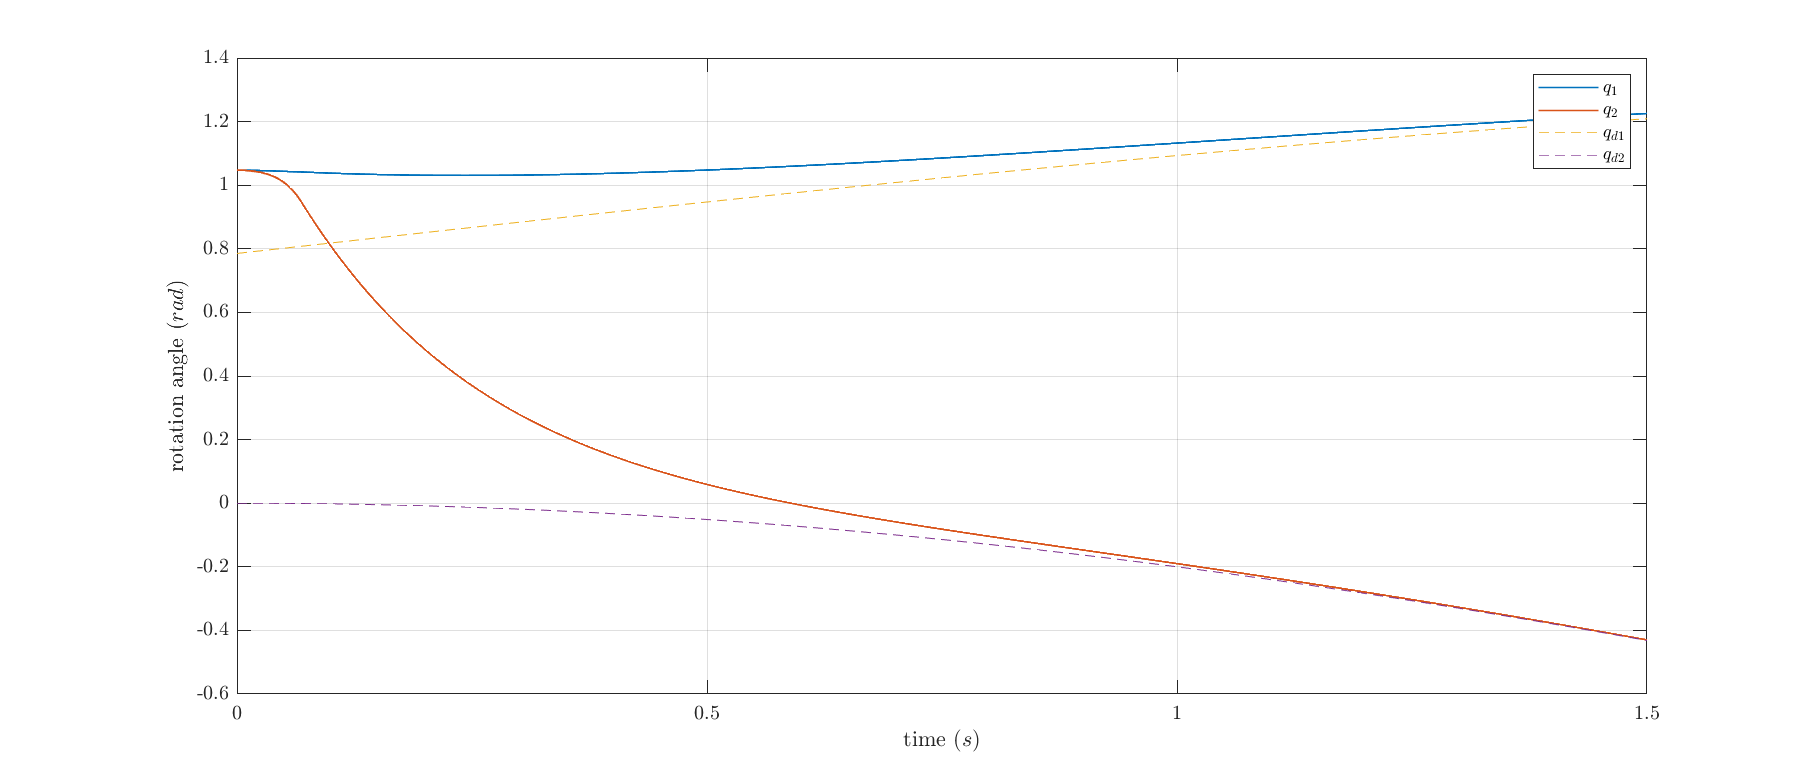
\includegraphics[width=15cm]{fig/sim2/q.png}
    \caption{Rotation angles with respect to time}
\end{figure}
\begin{figure}[H]
    \centering
    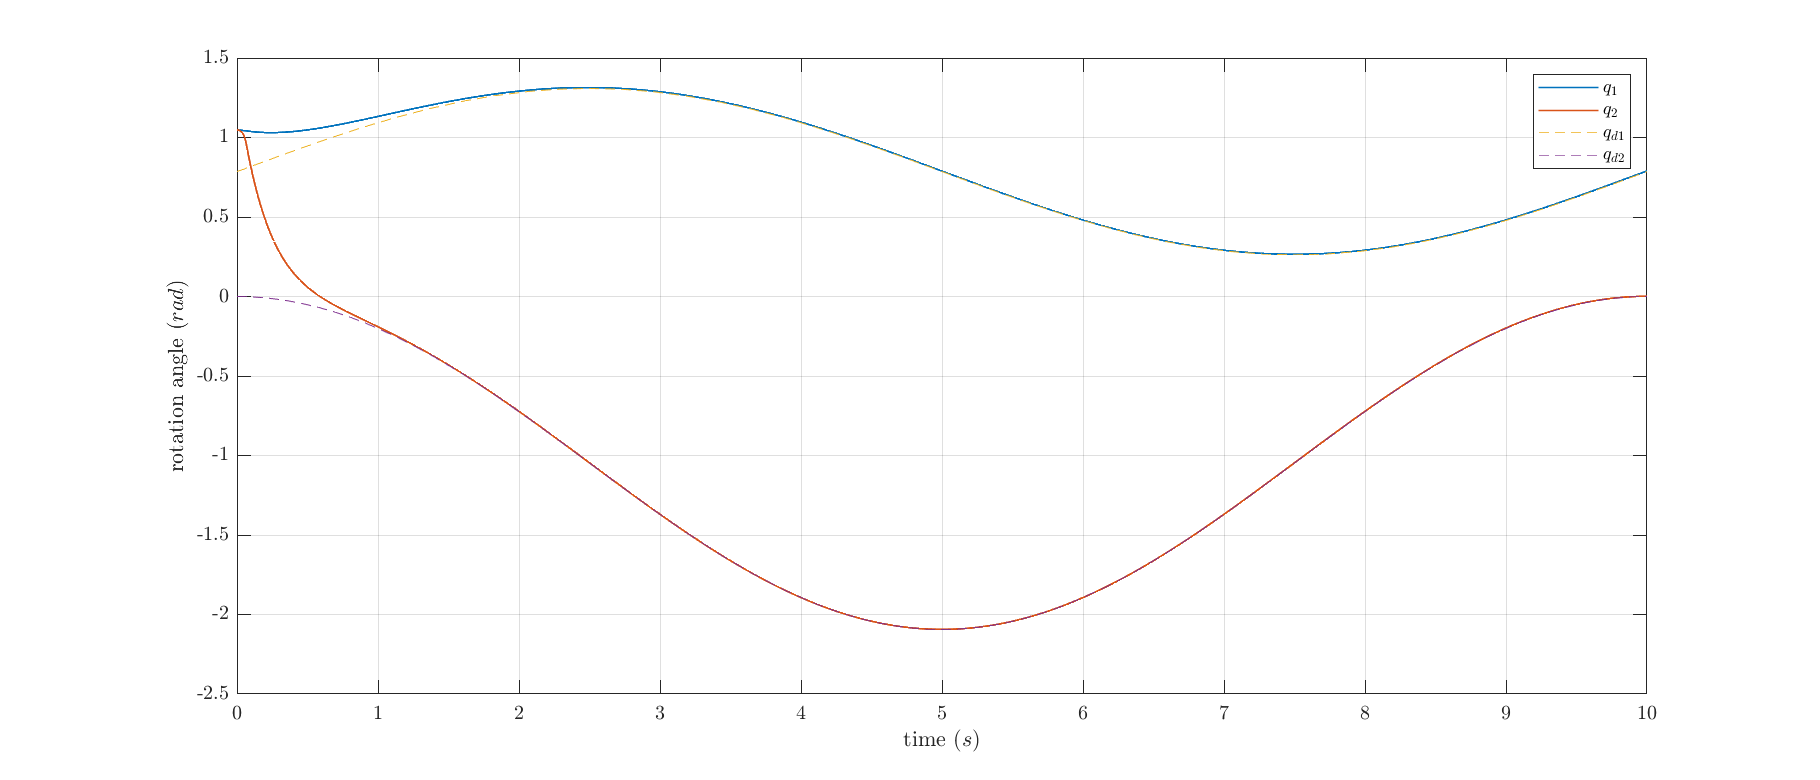
\includegraphics[width=15cm]{fig/sim2/qlong.png}
    \caption{Rotation angles with respect to time - long scale}
\end{figure}
\begin{figure}[H]
    \centering
    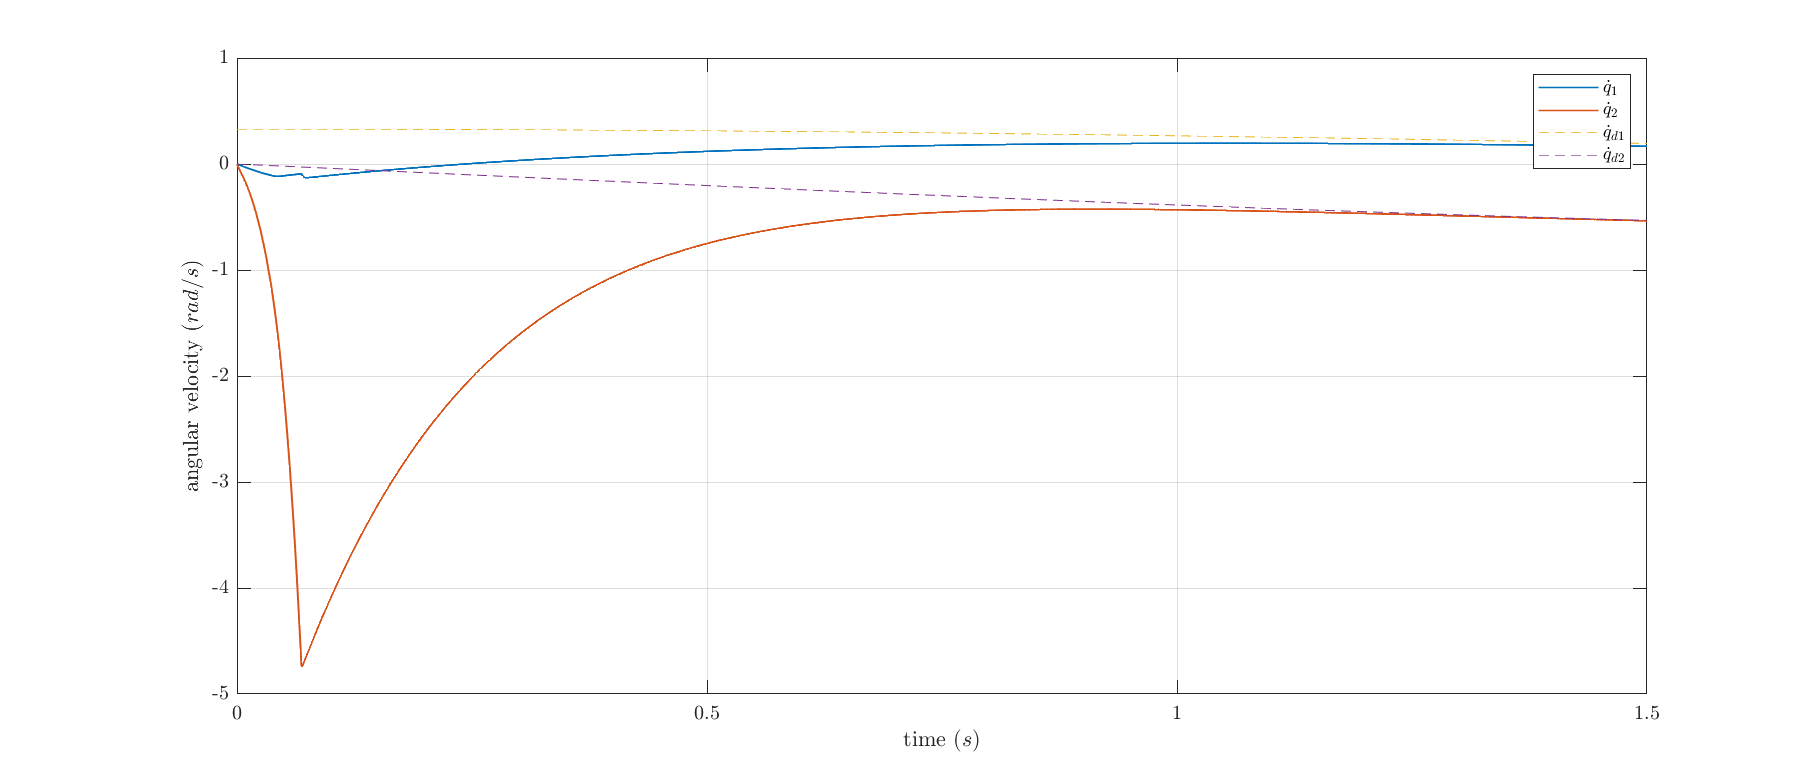
\includegraphics[width=15cm]{fig/sim2/qdot.png}
    \caption{Angular velocities with respect to time}
\end{figure}
\begin{figure}[H]
    \centering
    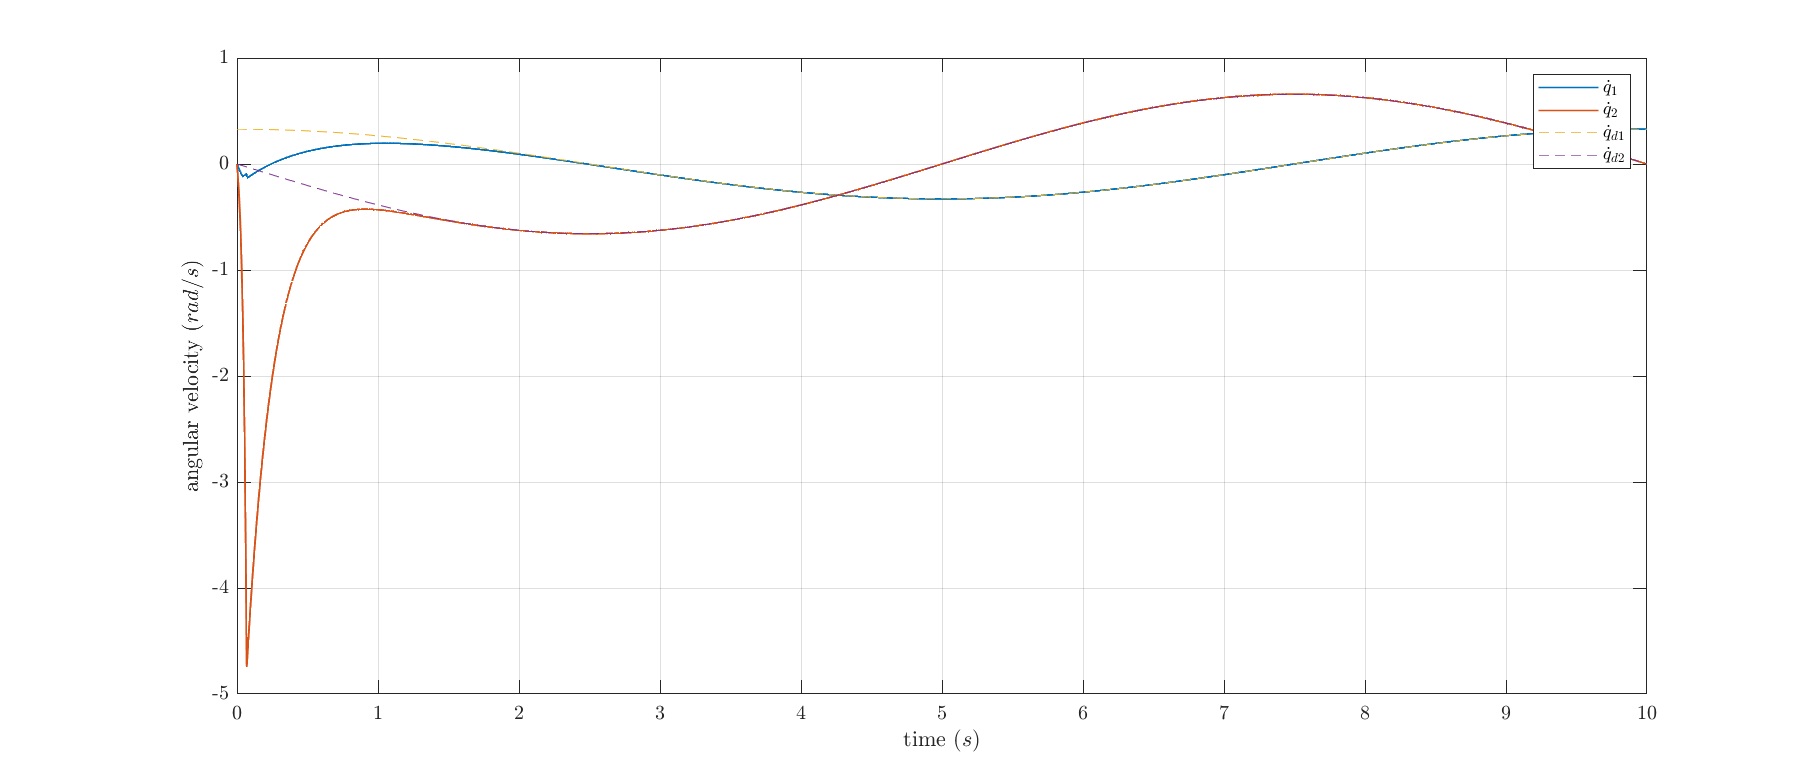
\includegraphics[width=15cm]{fig/sim2/qdotlong.png}
    \caption{Angular velocities with respect to time - long scale}
\end{figure}
\begin{figure}[H]
    \centering
    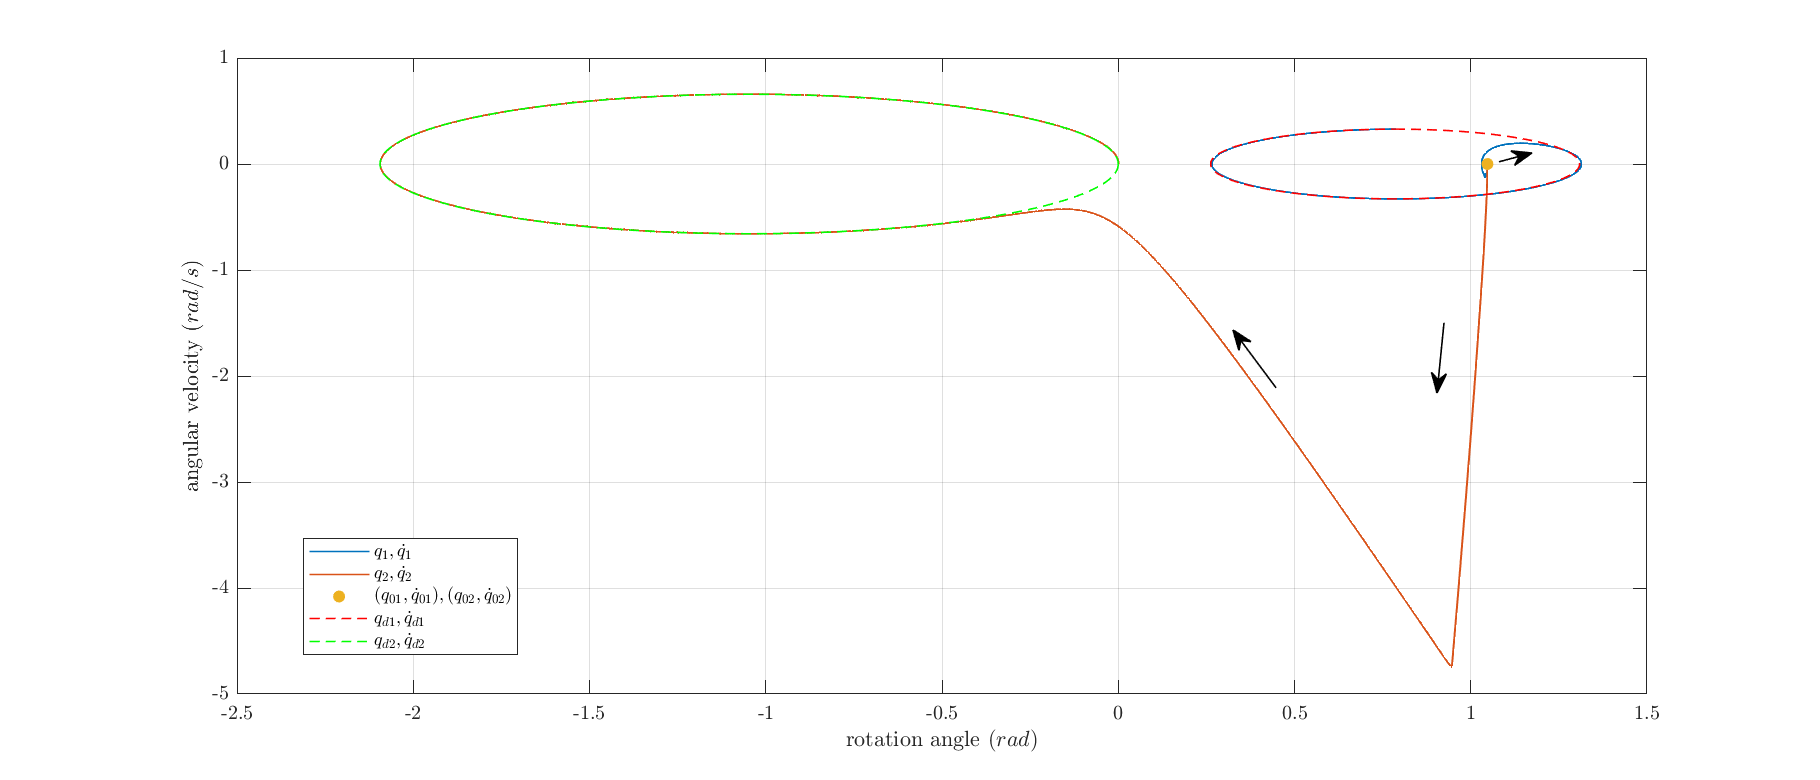
\includegraphics[width=15cm]{fig/sim2/phaseplanelong.png}
    \caption{Phase plane of system states - long scale}
\end{figure}
\begin{figure}[H]
    \centering
    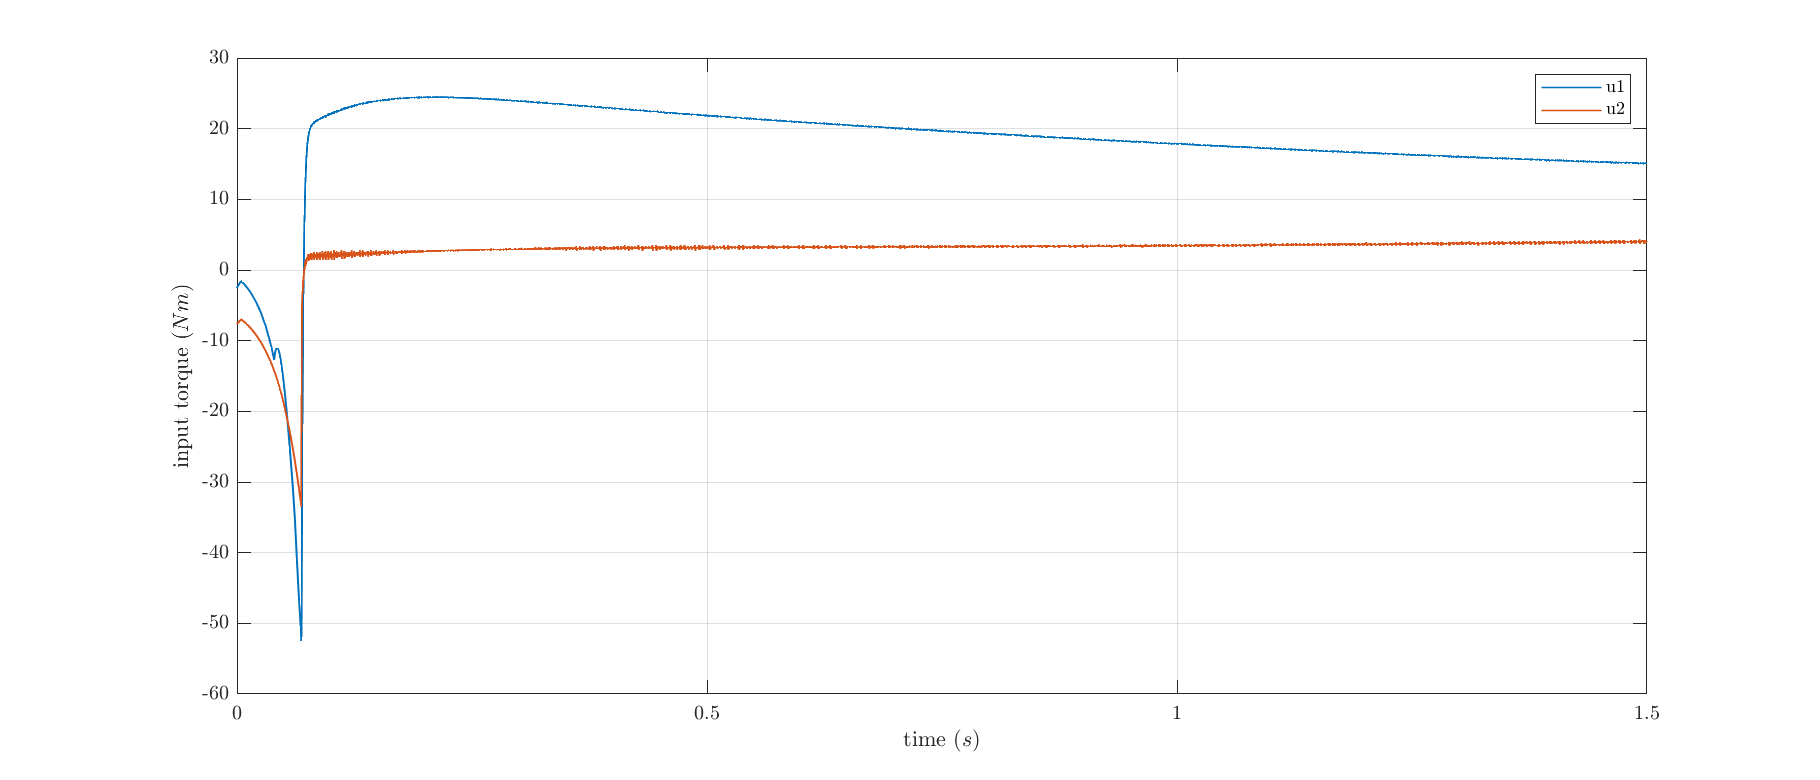
\includegraphics[width=15cm]{fig/sim2/u.png}
    \caption{Control input with respect to time}
\end{figure}
\begin{figure}[H]
    \centering
    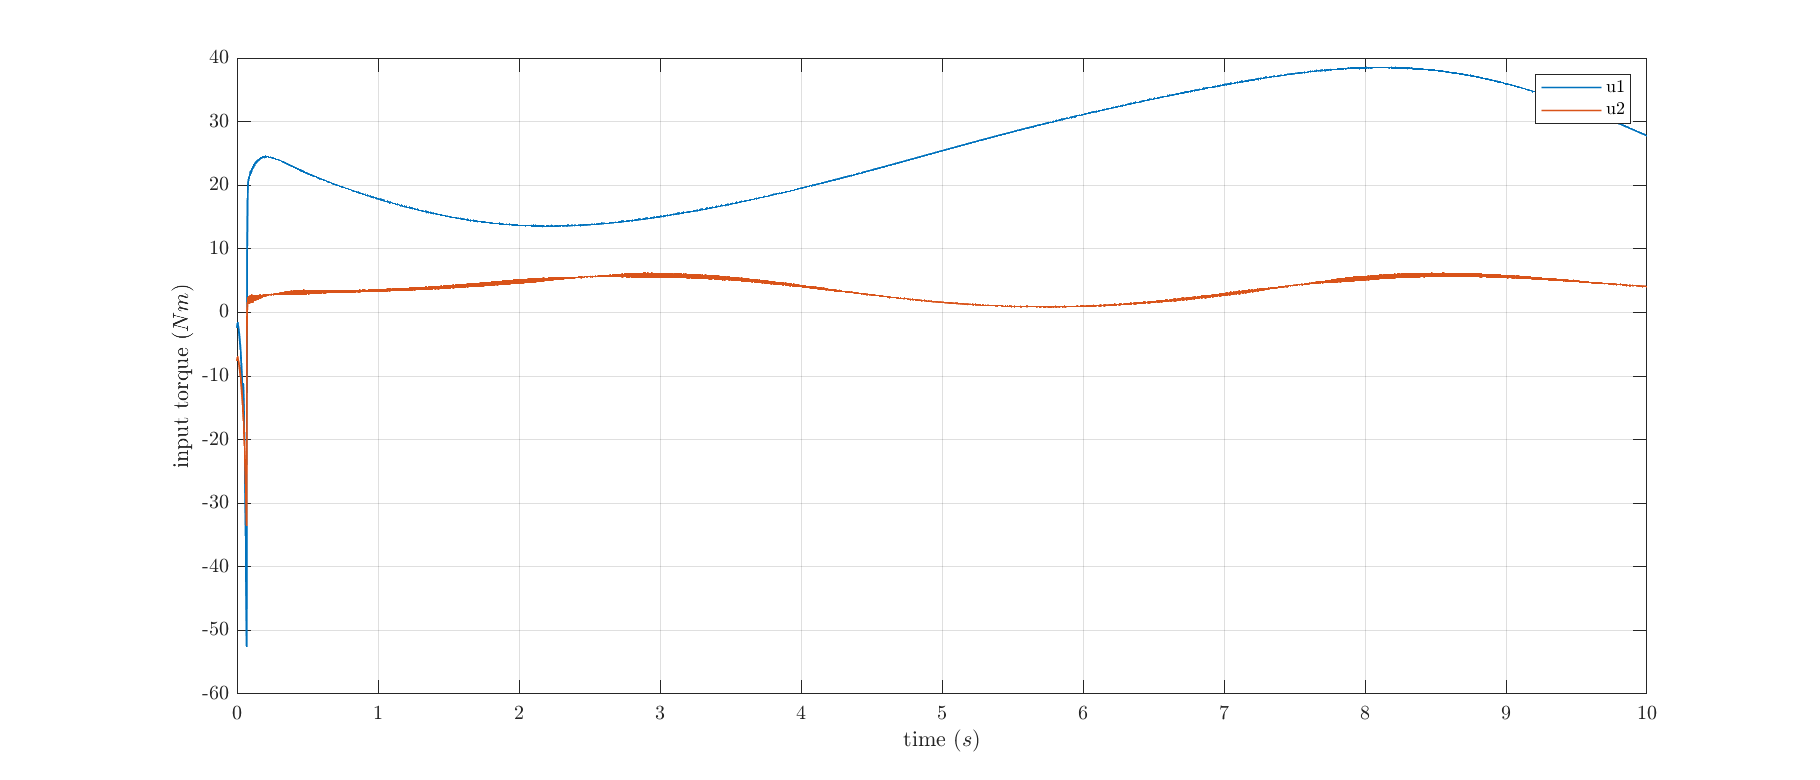
\includegraphics[width=15cm]{fig/sim2/ulong.png}
    \caption{Control input with respect to time - long sclae}
\end{figure}
\begin{figure}[H]
    \centering
    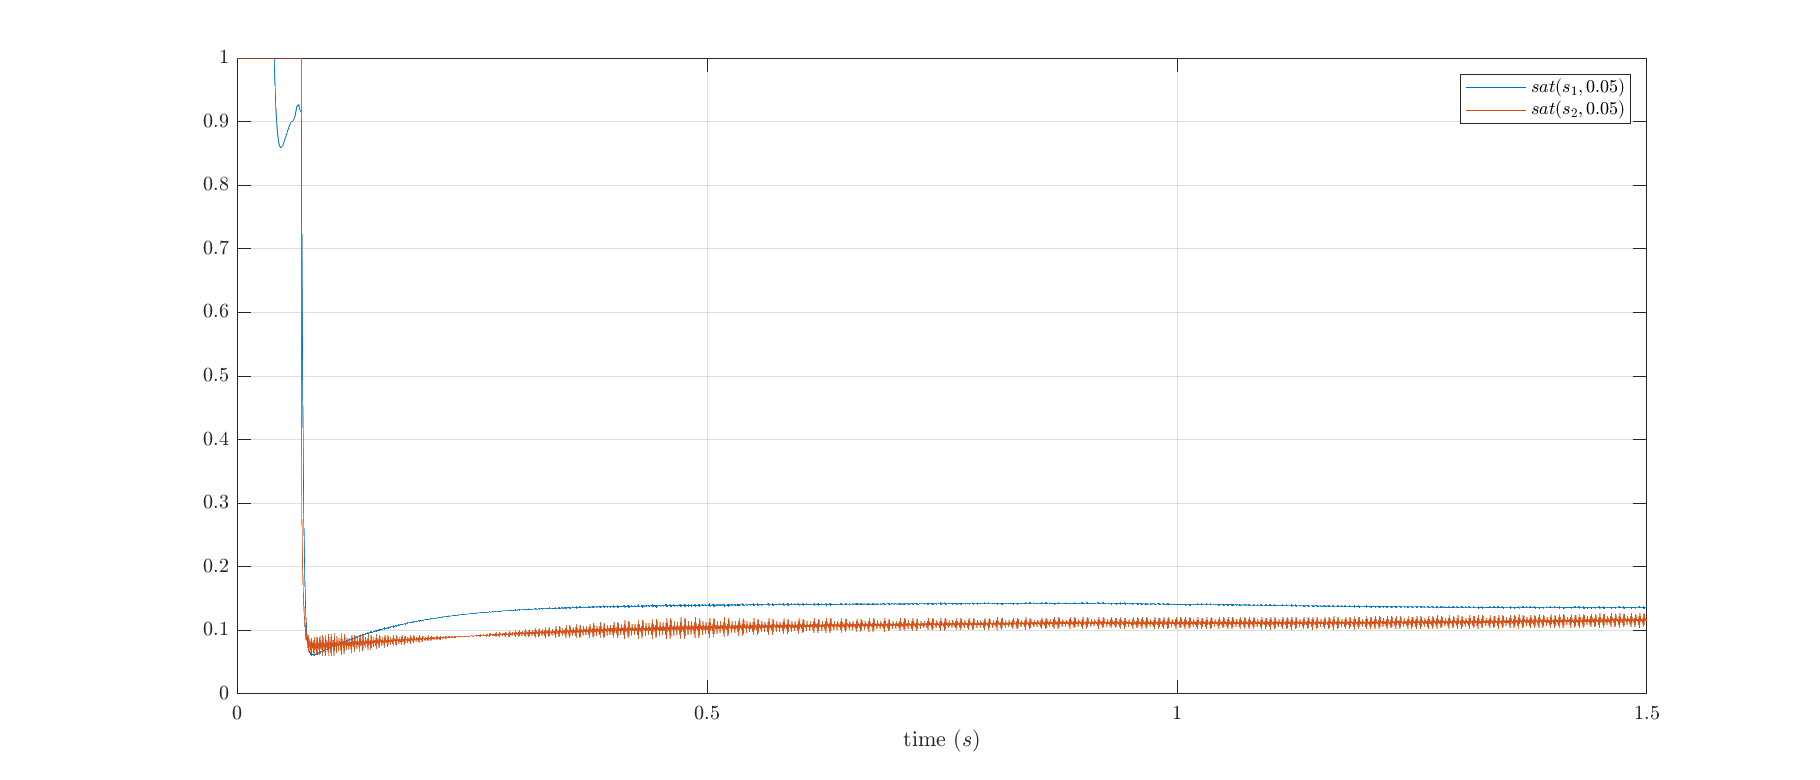
\includegraphics[width=15cm]{fig/sim2/sat.png}
    \caption{Saturation function of controller with respect to time}
\end{figure}
\begin{figure}[H]
    \centering
    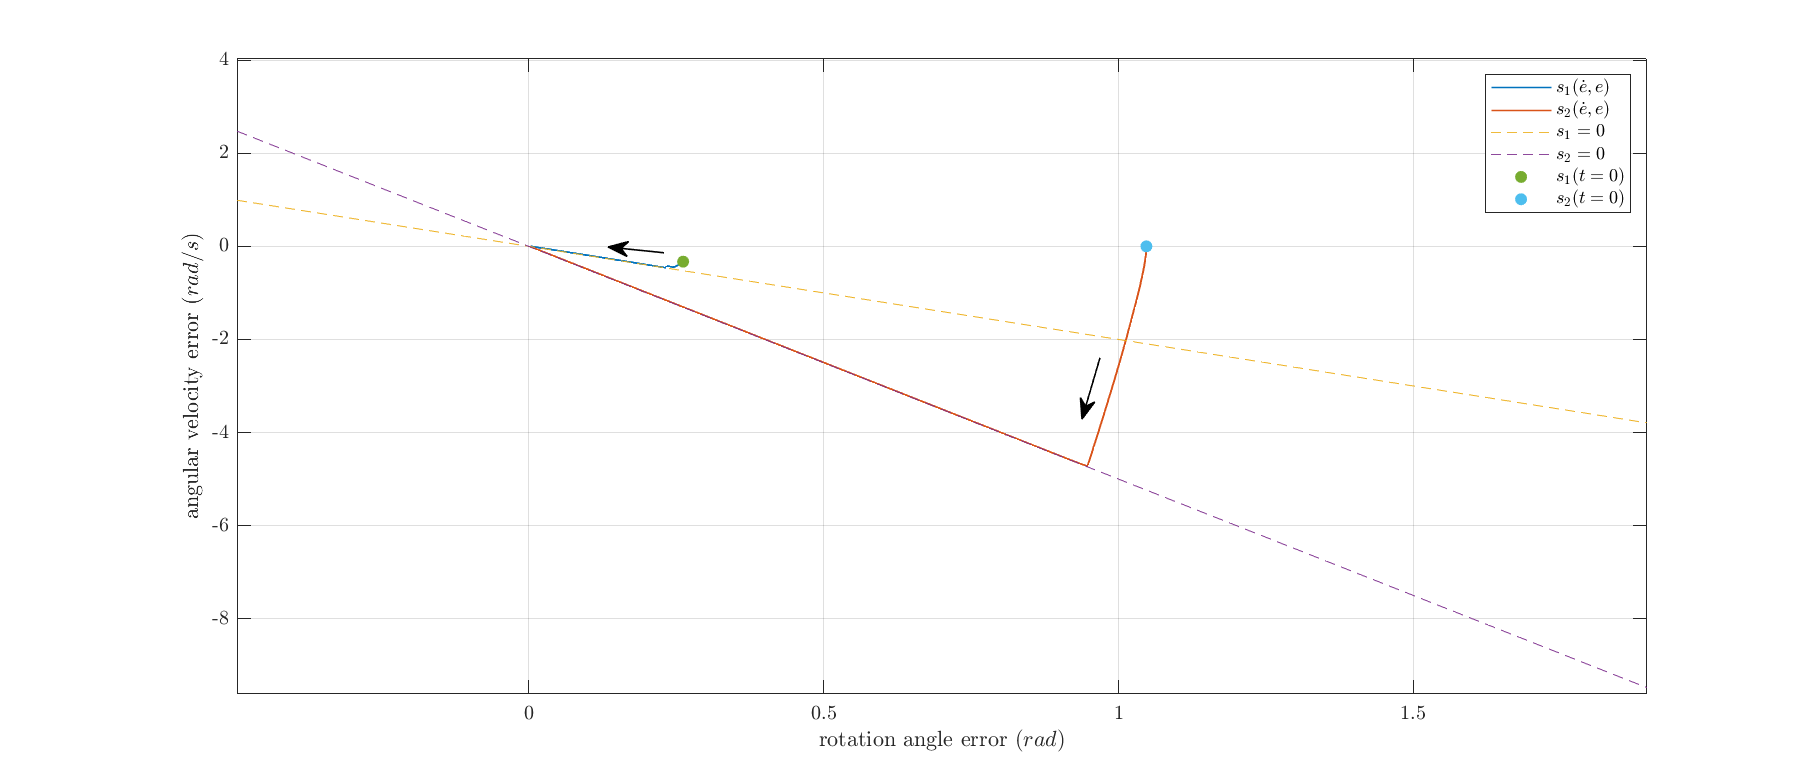
\includegraphics[width=15cm]{fig/sim2/slidinglong.png}
    \caption{Convergence to sliding surface - long scale}
\end{figure}
\begin{figure}[H]
    \centering
    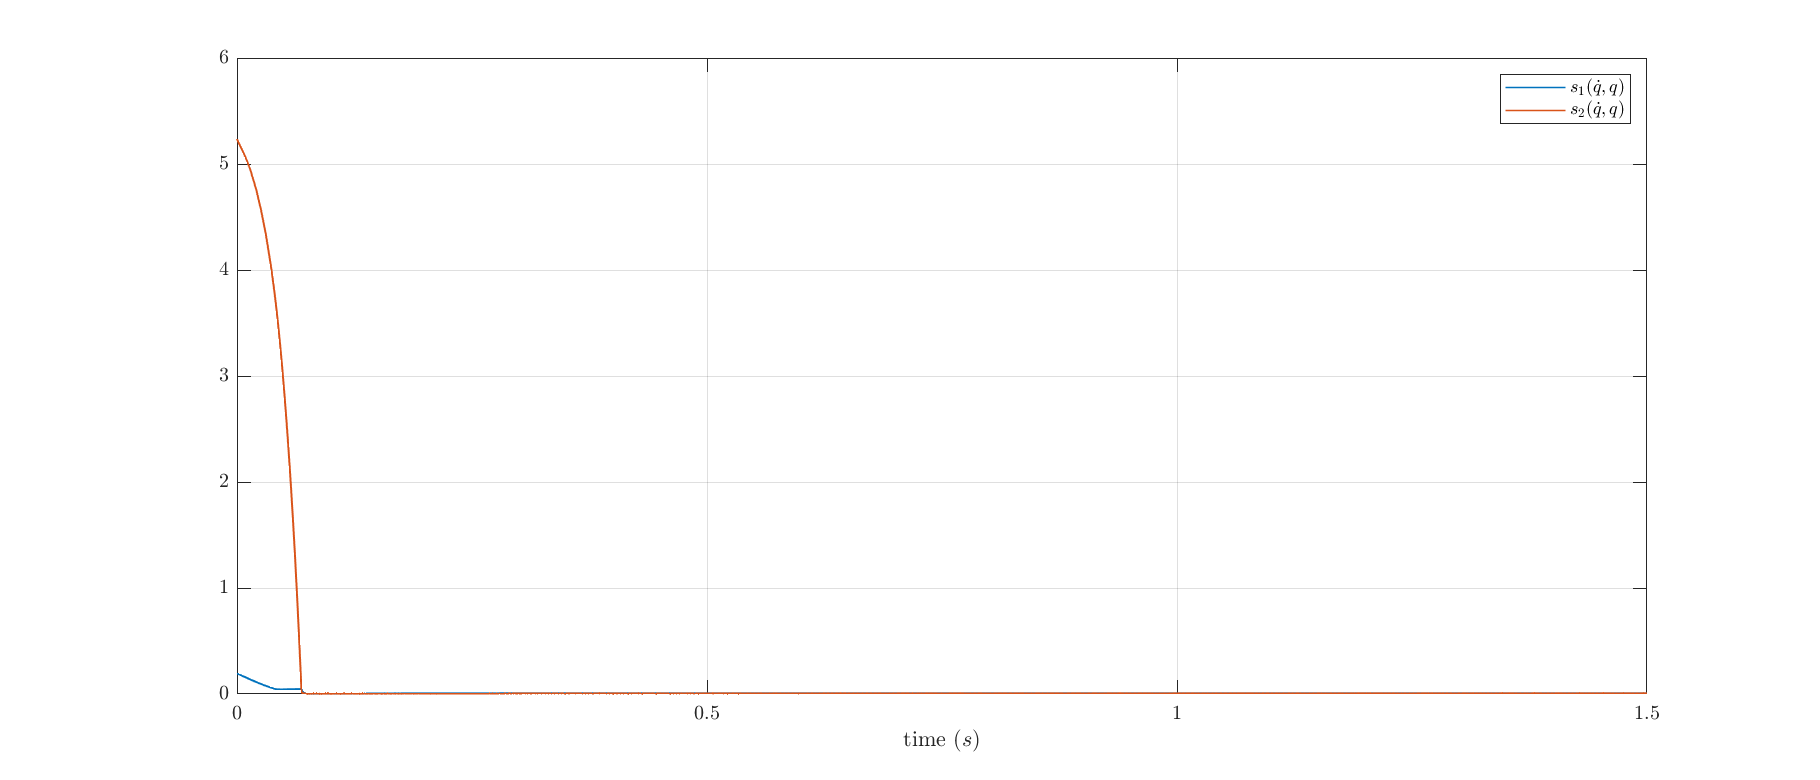
\includegraphics[width=15cm]{fig/sim2/s.png}
    \caption{Surface $s(\dot{q}, q)$ with respect to time}
\end{figure}
\begin{figure}[H]
    \centering
    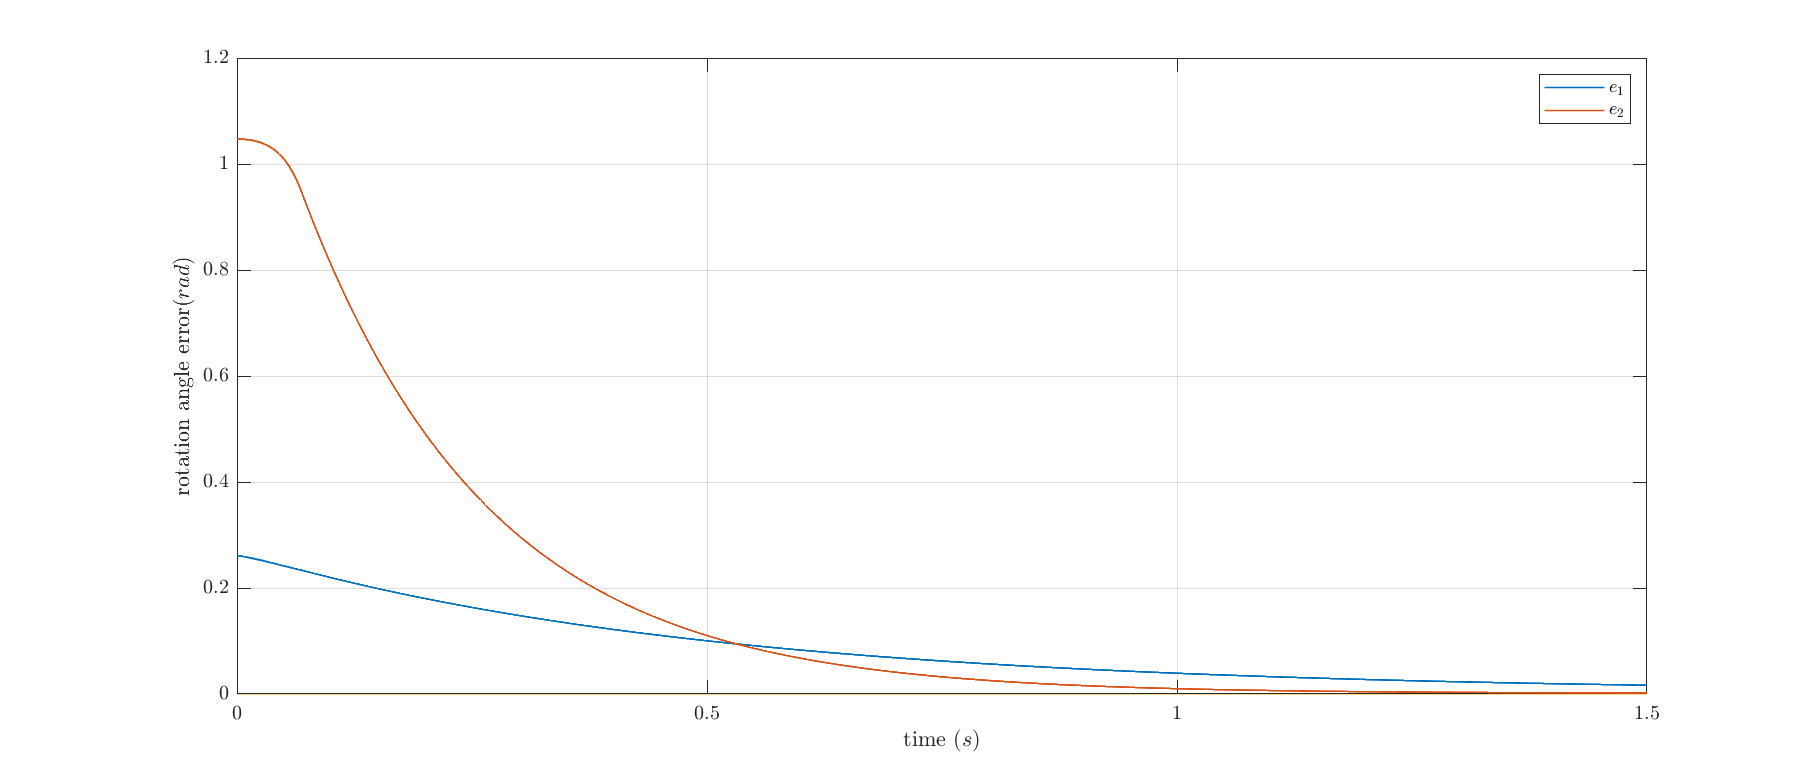
\includegraphics[width=15cm]{fig/sim2/e.png}
    \caption{State error with respect to time}
\end{figure}
\begin{figure}[H]
    \centering
    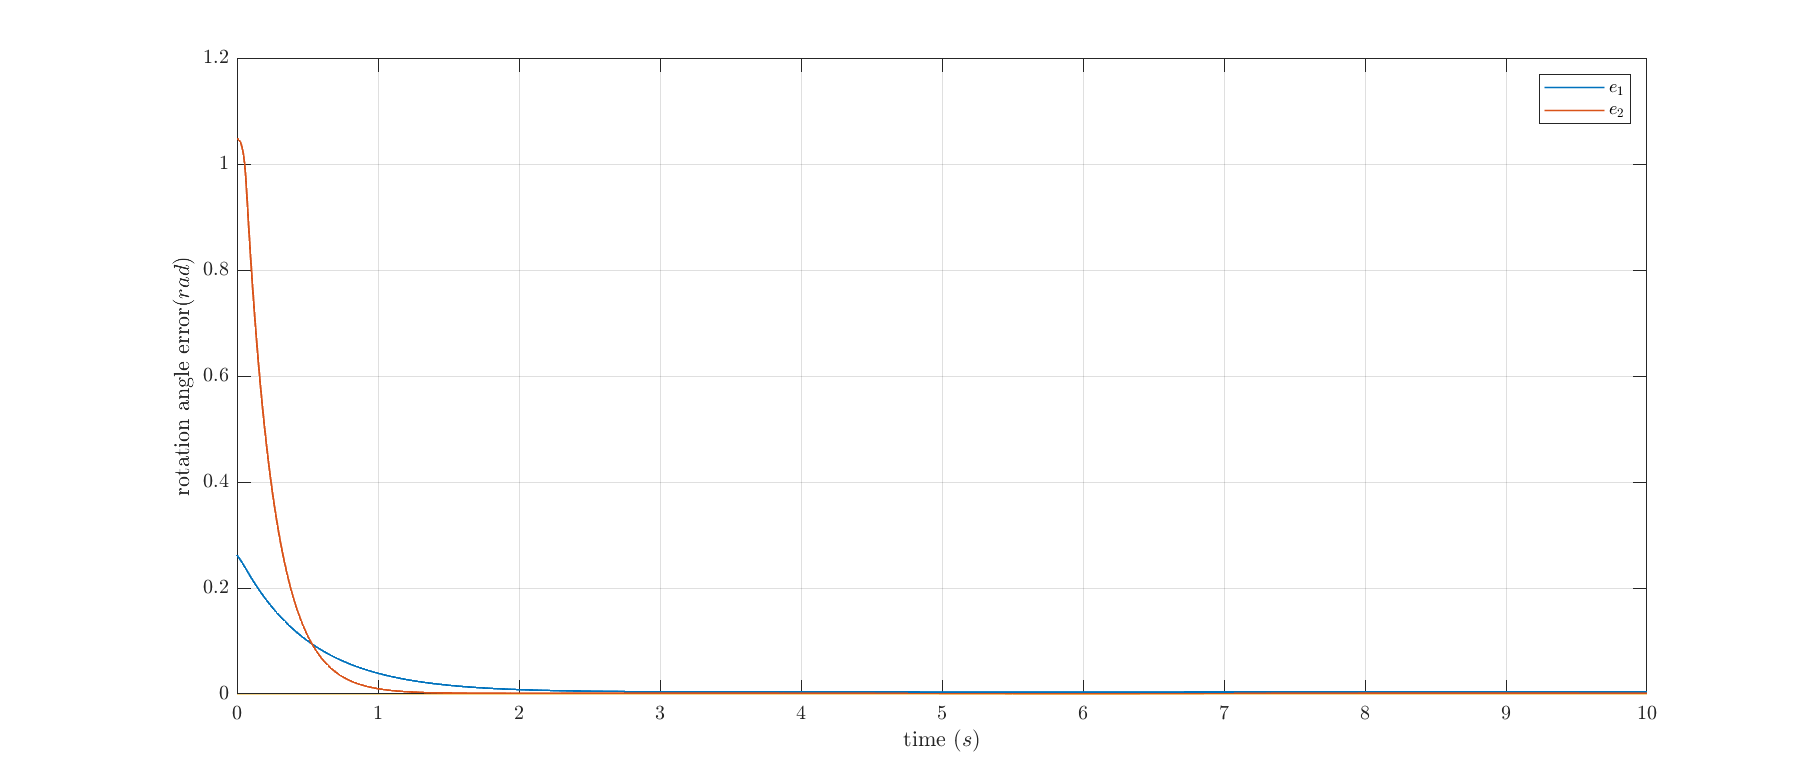
\includegraphics[width=15cm]{fig/sim2/elong.png}
    \caption{State error with respect to time - long scale}
\end{figure}

\begin{itemize}
    \item From figures 17, 18, 19 and 20 we can export that the system states track very satisfactorily the 
    desired state orbits and they converge to these orbits in less than 1 second.
    \item In figure 21, we can observe the phase plane of the system states as they converge to the 
    desired orbits. Since they reach these orbits, they keep moving in them.
    \item Figures 22 and 23 prove that the control input is satisfactorily bounded and the maximum power is not too high.
    \item We can conclude that all the signals in the closed loop are bounded.
    \item In figure 24, we can see that the saturation function becomes much more stable, by the time that the 
    system reaches the $| \varepsilon |$ bounds (figure 26). However, there is still chattering in the saturation function, 
    which leads the control input and thus, the system states to slight chattering too.
    \item The convergence of the system to the $s=0$ surface can be noticed in figure 25. In constrast with the 
    \textit{regulation} problem, this time we choose different values for $\lambda_1$ and $\lambda_2$, which results in two different lines for 
    $s_1=0$ and $s_2=0$. As we can see in figure 25, each component of $s(\dot{e}, e)$ converges to a different \textit{sliding line}. 
    \item In figure 26, we can see the convergence of the system to $s=0$ with respect to time. When $s(\dot{e}, e)$ reaches close to 
    zero, the state error starts decreasing (figure 27), as the error slides through the \textit{sliding surface}.
\end{itemize}

\newpage
\subsubsection{Parameter $c$ analysis}
As we explained before, the parameter $c$ defines the speed of convergence to the \textit{sliding surface}.
We present the results for $c=1$ and $c=25$ separately, with constant $\lambda_1 = 2$ and $\lambda_2 = 5$:
\begin{figure}[H]
    \centering
    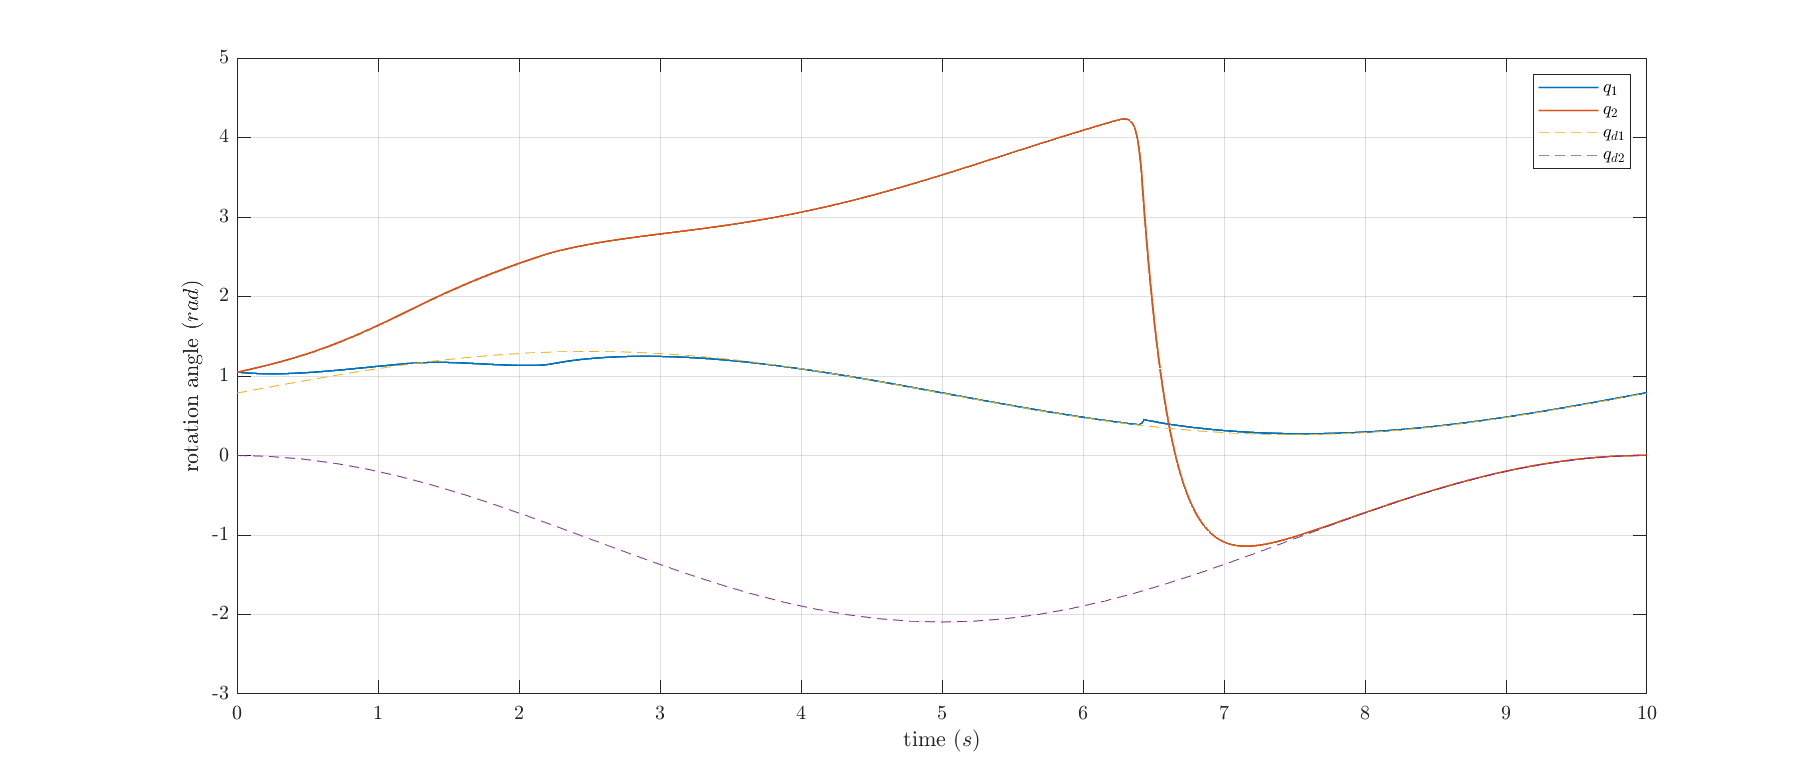
\includegraphics[width=15cm]{fig/sim2/c1/q1.png}
    \caption{Rotation angles with respect to time for $c=1$}
\end{figure}
\begin{figure}[H]
    \centering
    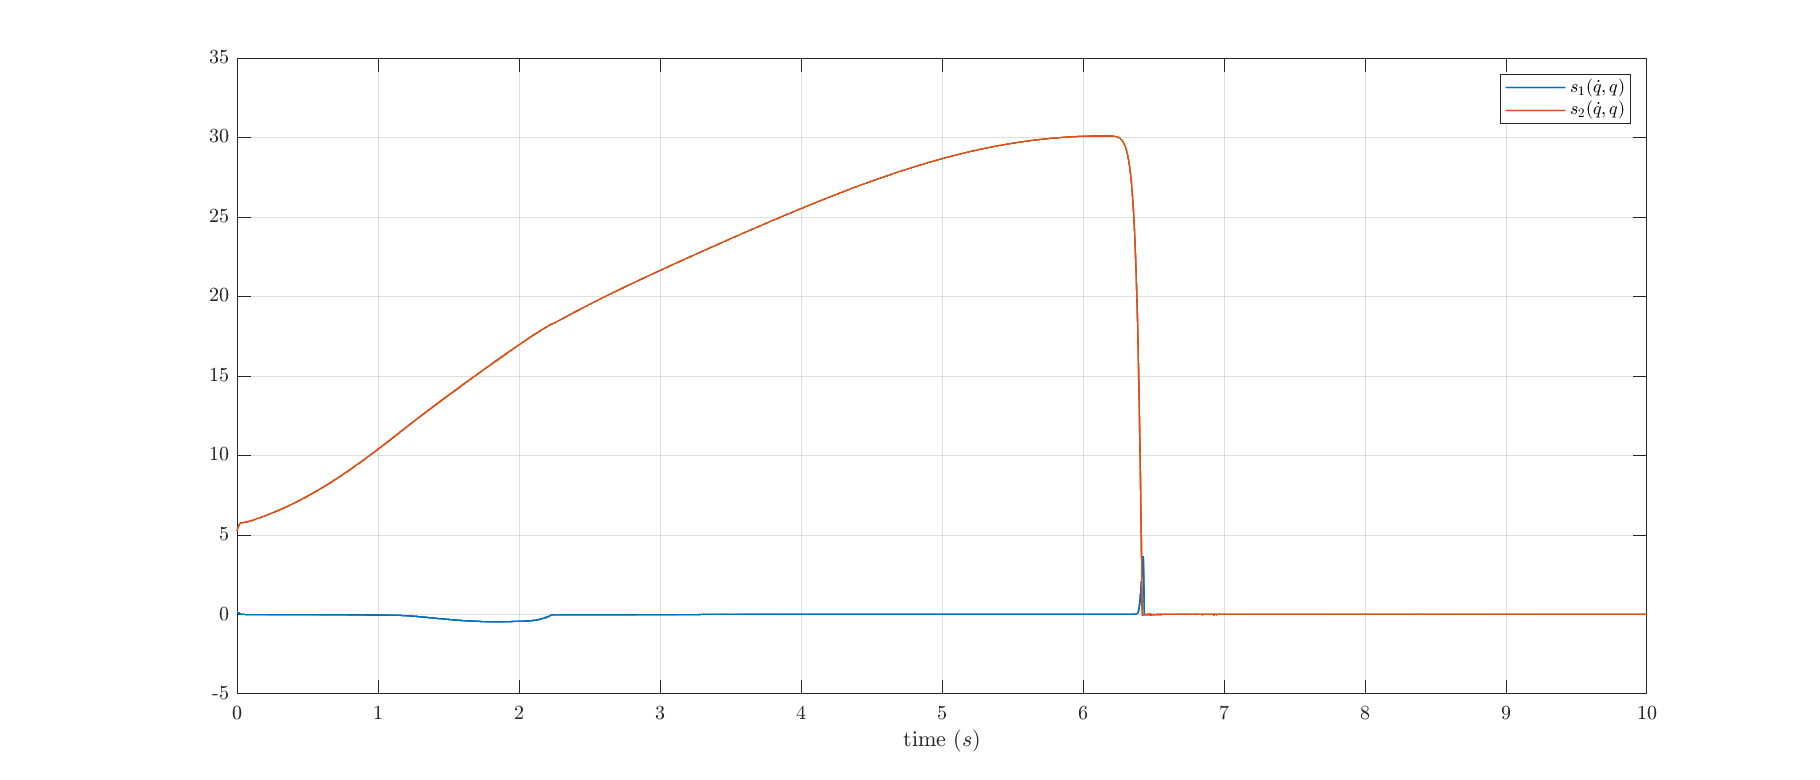
\includegraphics[width=15cm]{fig/sim2/c1/s1.png}
    \caption{Surface $s(\dot{q}, q)$ with respect to time for $c=1$}
\end{figure}
\begin{figure}[H]
    \centering
    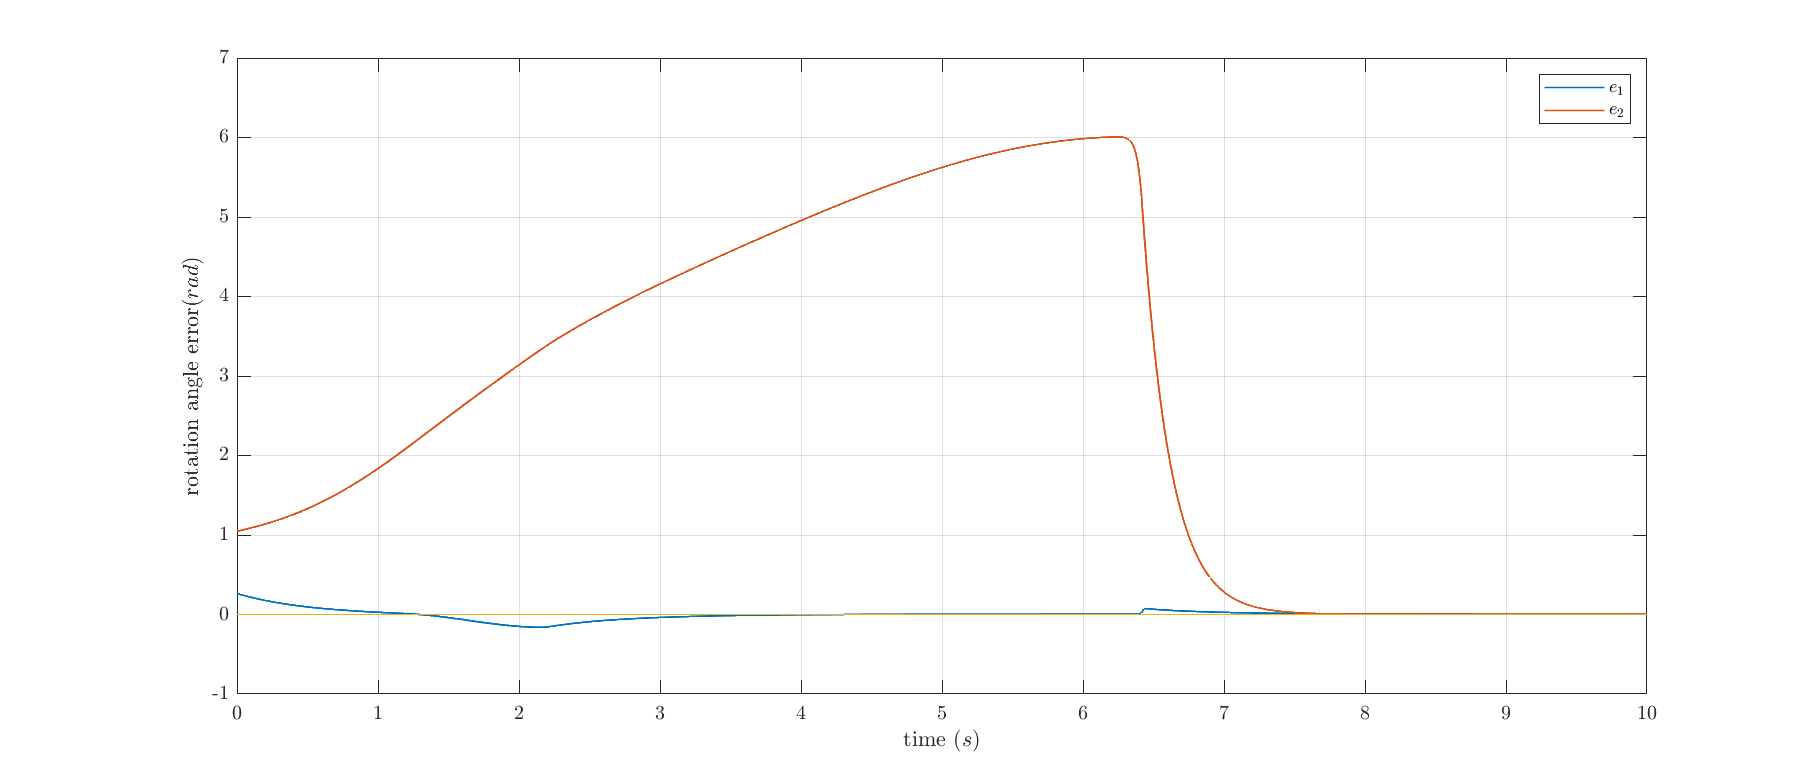
\includegraphics[width=15cm]{fig/sim2/c1/e1.png}
    \caption{State error with respect to time for $c=1$}
\end{figure}
\begin{figure}[H]
    \centering
    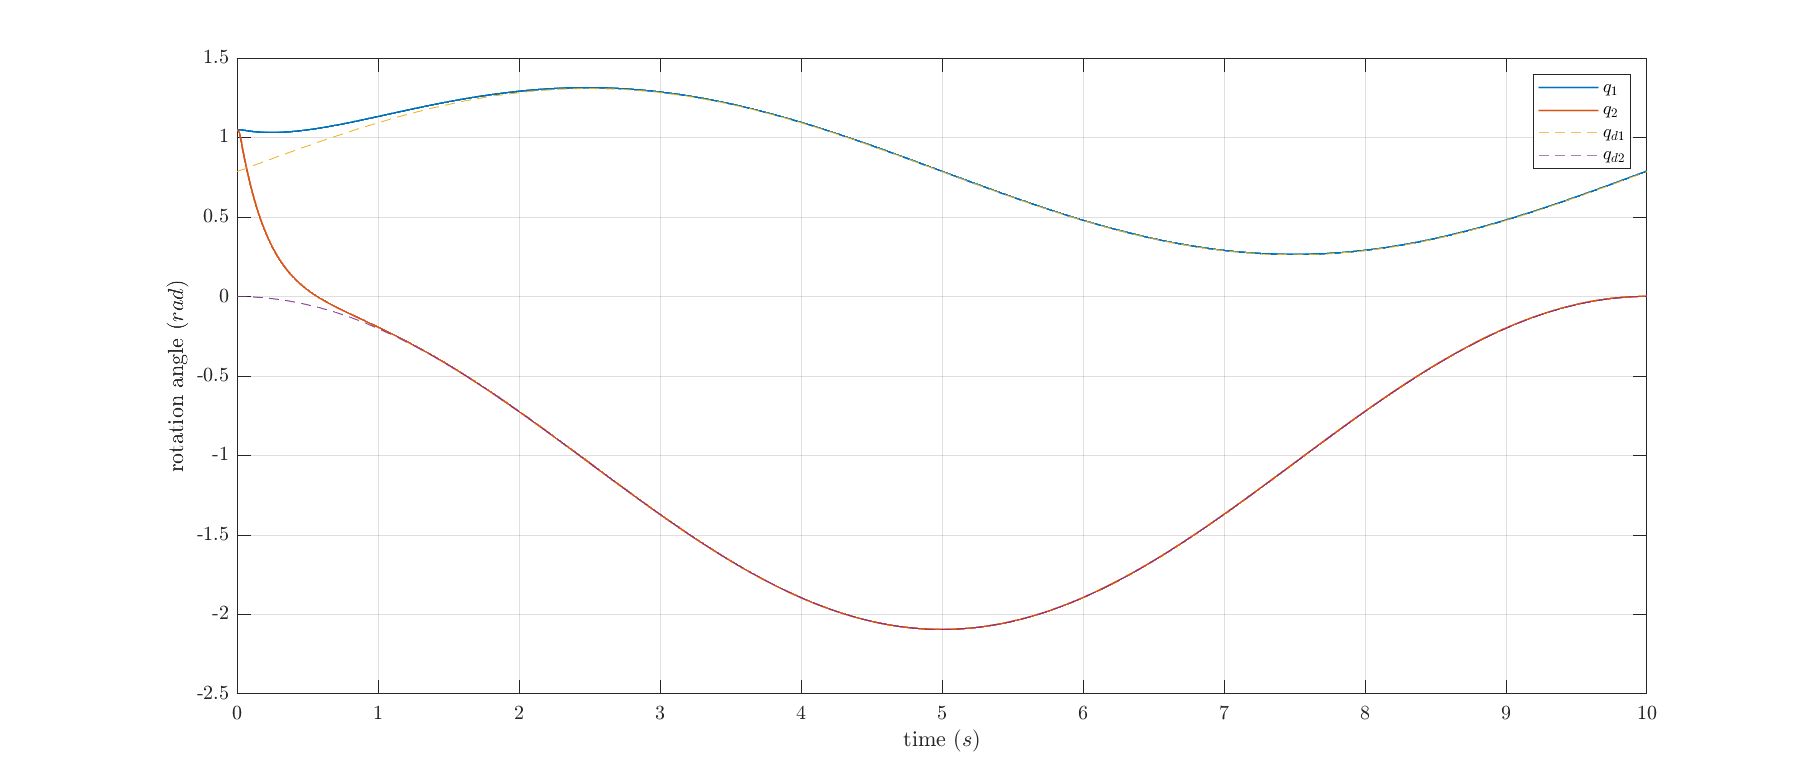
\includegraphics[width=15cm]{fig/sim2/c25/q25.png}
    \caption{Rotation angles with respect to time for $c=25$}
\end{figure}
\begin{figure}[H]
    \centering
    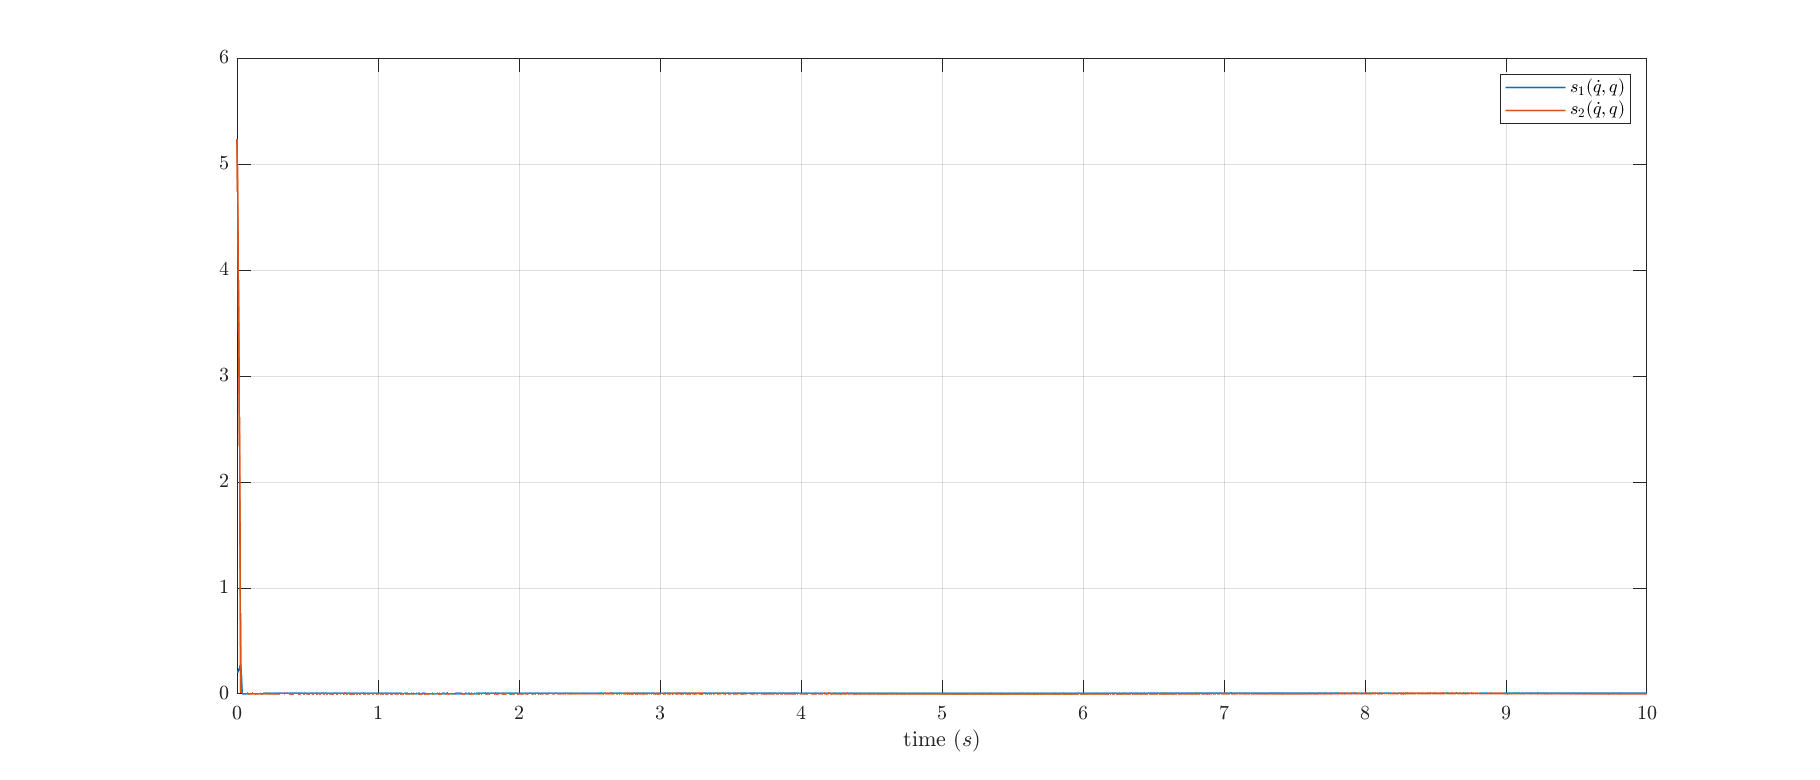
\includegraphics[width=15cm]{fig/sim2/c25/s25.png}
    \caption{Surface $s(\dot{q}, q)$ with respect to time for $c=25$}
\end{figure}
\begin{figure}[H]
    \centering
    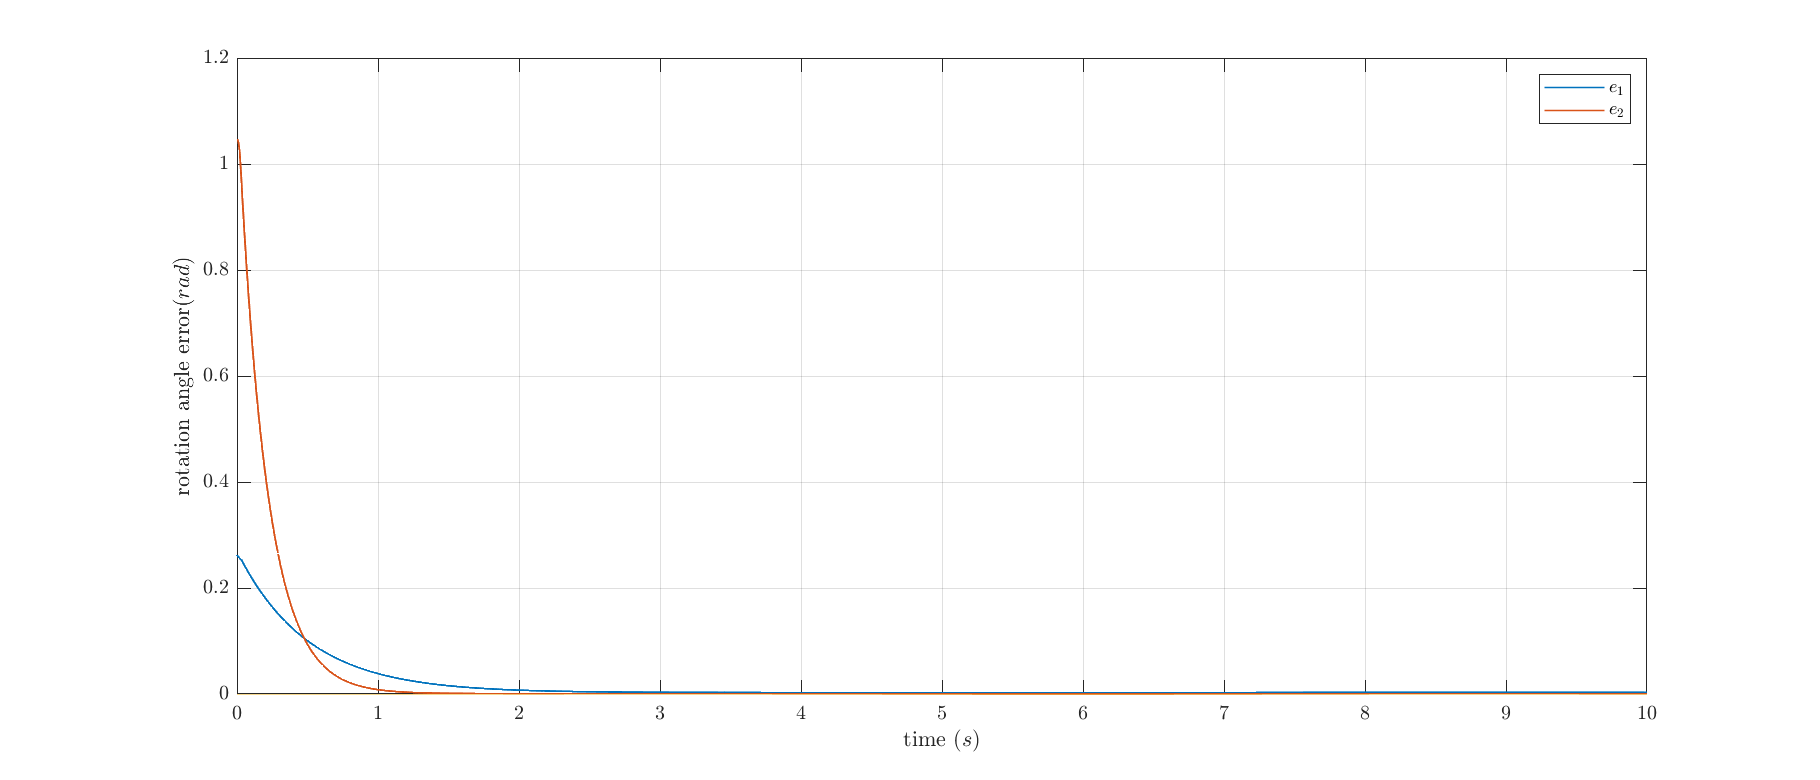
\includegraphics[width=15cm]{fig/sim2/c25/e25.png}
    \caption{State error with respect to time for $c=25$}
\end{figure}

\noindent\hspace{-2pt}
Through figures 29, 30 and 31, we validate our theoretical estimations, as the convergence to the 
\textit{sliding surface} is delayed for a lower value of $c$ ($c=1<10$). So, the error starts decreasing 
later in comparison with the case with the selected parameter $c$ ($c=10$).
For $c=25$, we can notice that the convergence has reached to saturation and cannot been improved further
as $c$ increases (figures 32, 34), although $s=0$ is reached earlier (figure 33).

\subsubsection{Parameter matrix $\Lambda$ analysis}
According to matrix $\Lambda$, we will firstly decrease the values of the matrix and set $\lambda_1 = 0.2$ 
and $\lambda_2 = 0.5$ with constant $c=10$. Subsequently, we will increase the values to $\lambda_1 = 10$ and $\lambda_2 = 20$. 
We present the results below:
\begin{figure}[H]
    \centering
    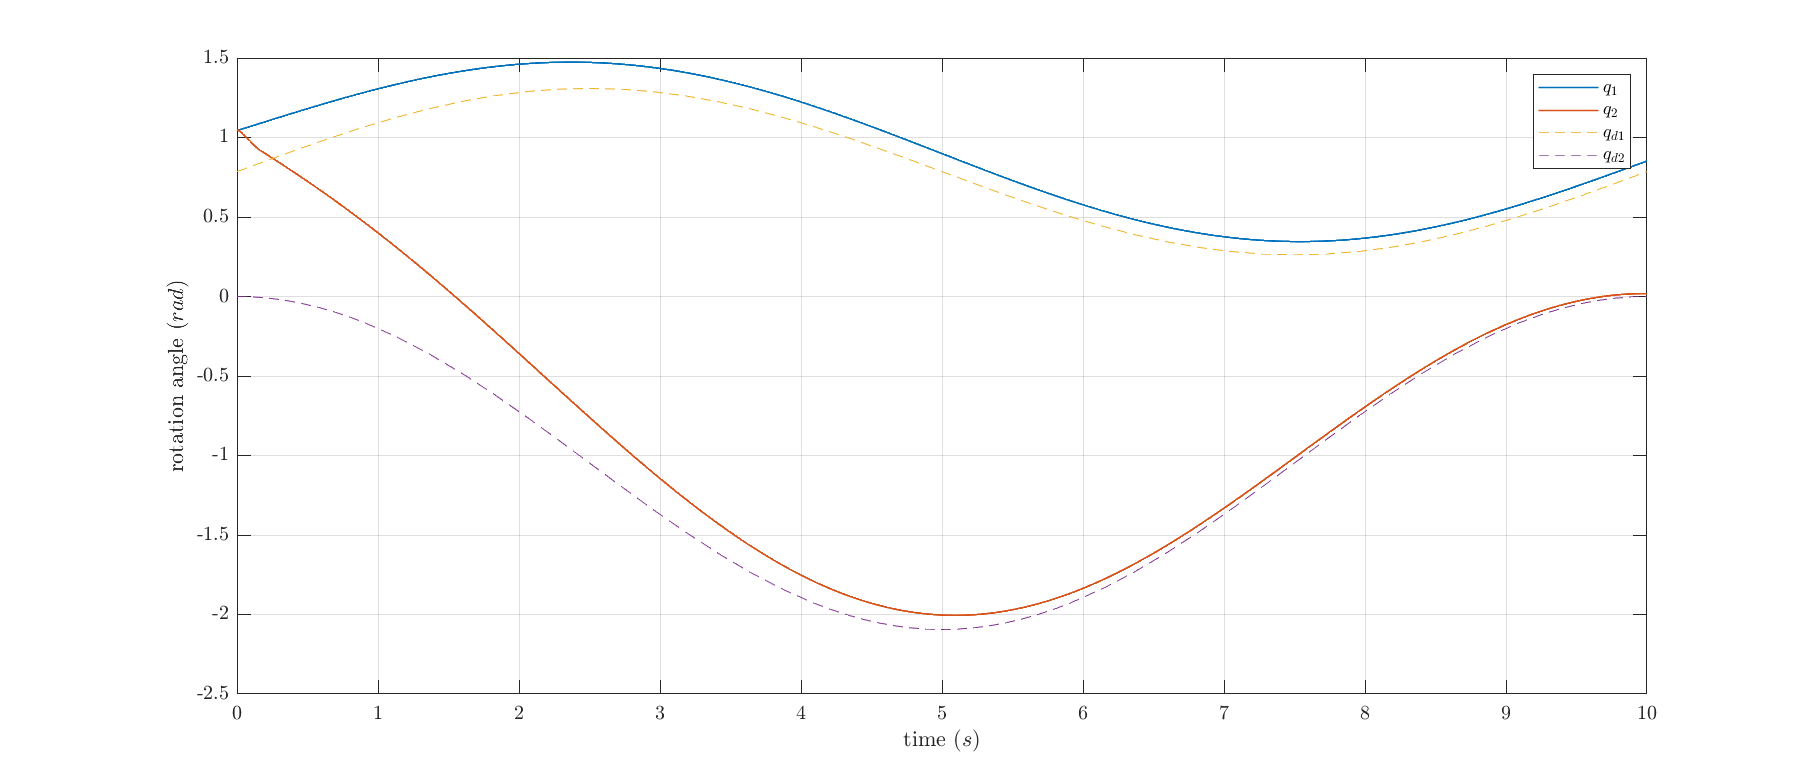
\includegraphics[width=15cm]{fig/sim2/ldecrease/qldecrease.png}
    \caption{Rotation angles with respect to time for $\lambda_1=0.2$ and $\lambda_2=0.5$}
\end{figure}
\begin{figure}[H]
    \centering
    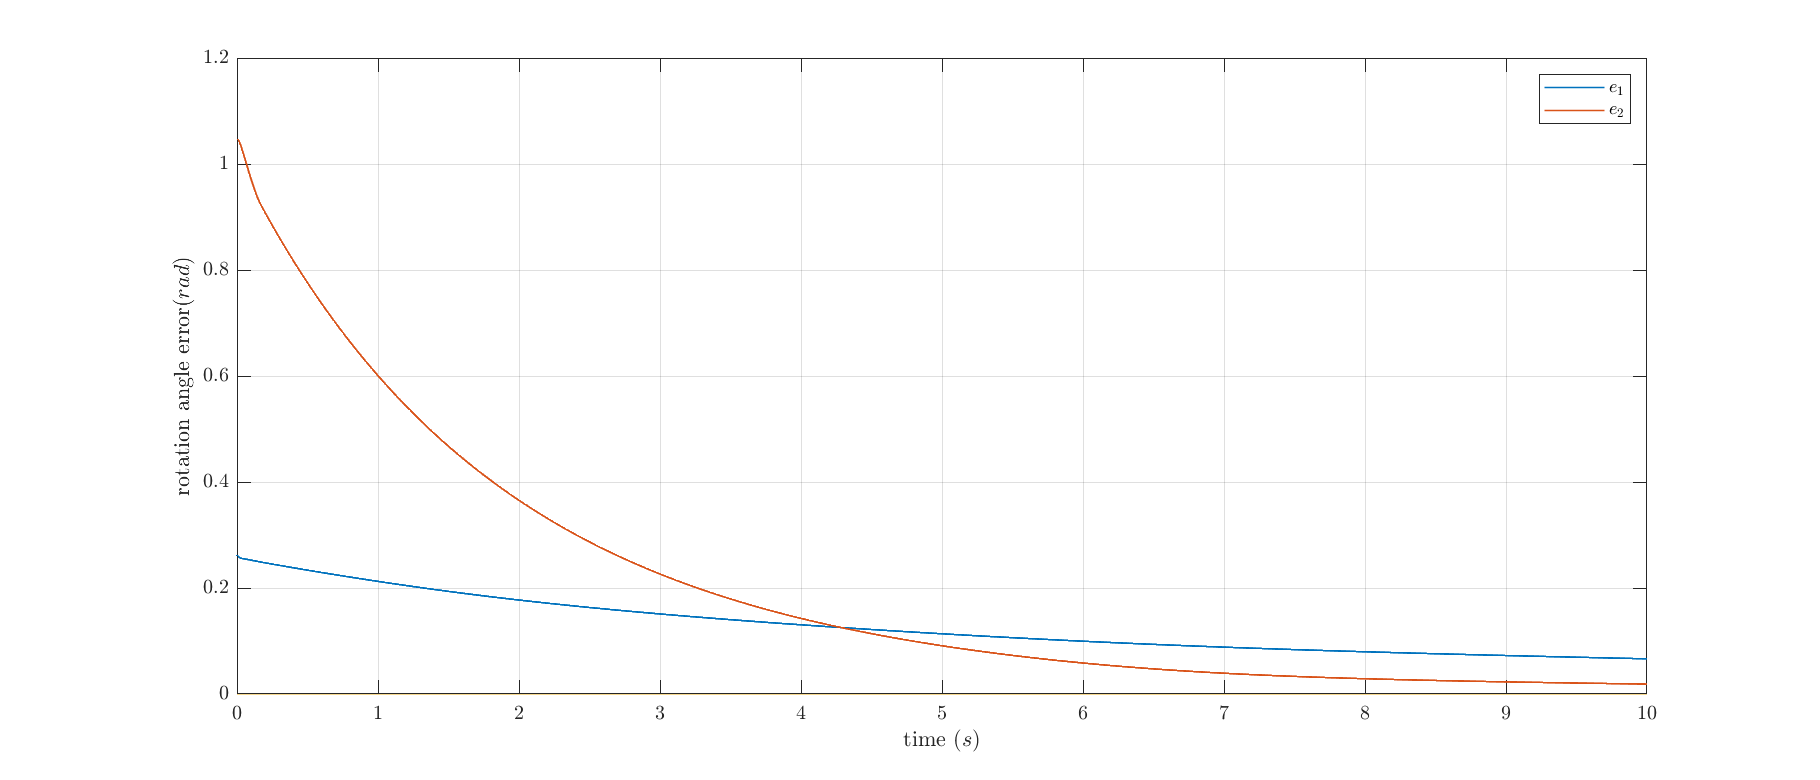
\includegraphics[width=15cm]{fig/sim2/ldecrease/eldecrease.png}
    \caption{State error with respect to time for $\lambda_1=0.2$ and $\lambda_2=0.5$}
\end{figure}
\begin{figure}[H]
    \centering
    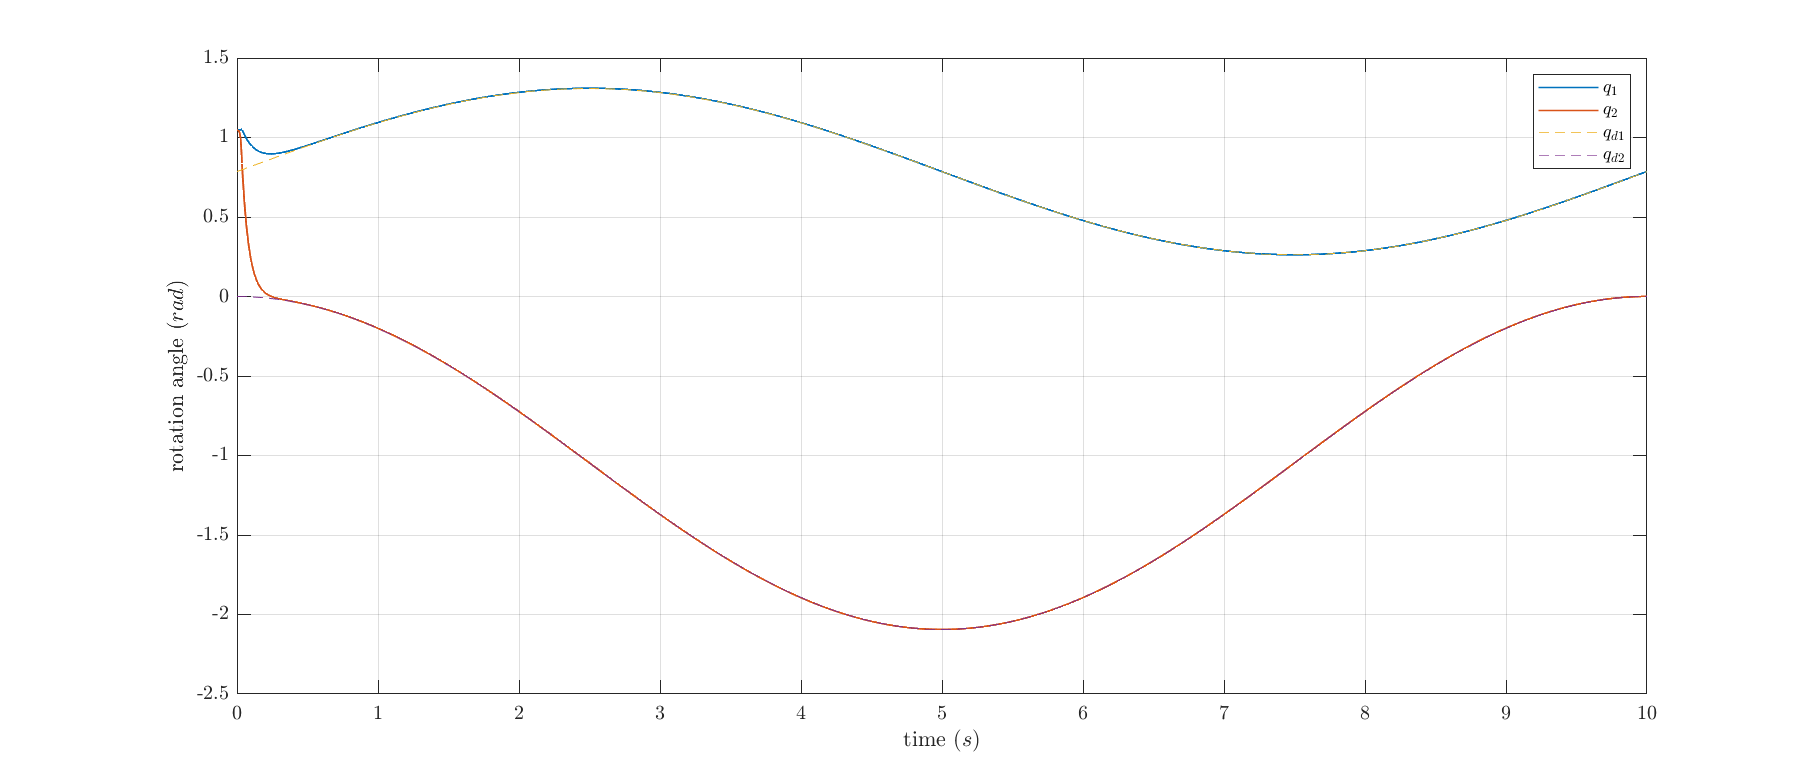
\includegraphics[width=15cm]{fig/sim2/lincrease/qlincrease.png}
    \caption{Rotation angles with respect to time for $\lambda_1=10$ and $\lambda_2=20$}
\end{figure}
\begin{figure}[H]
    \centering
    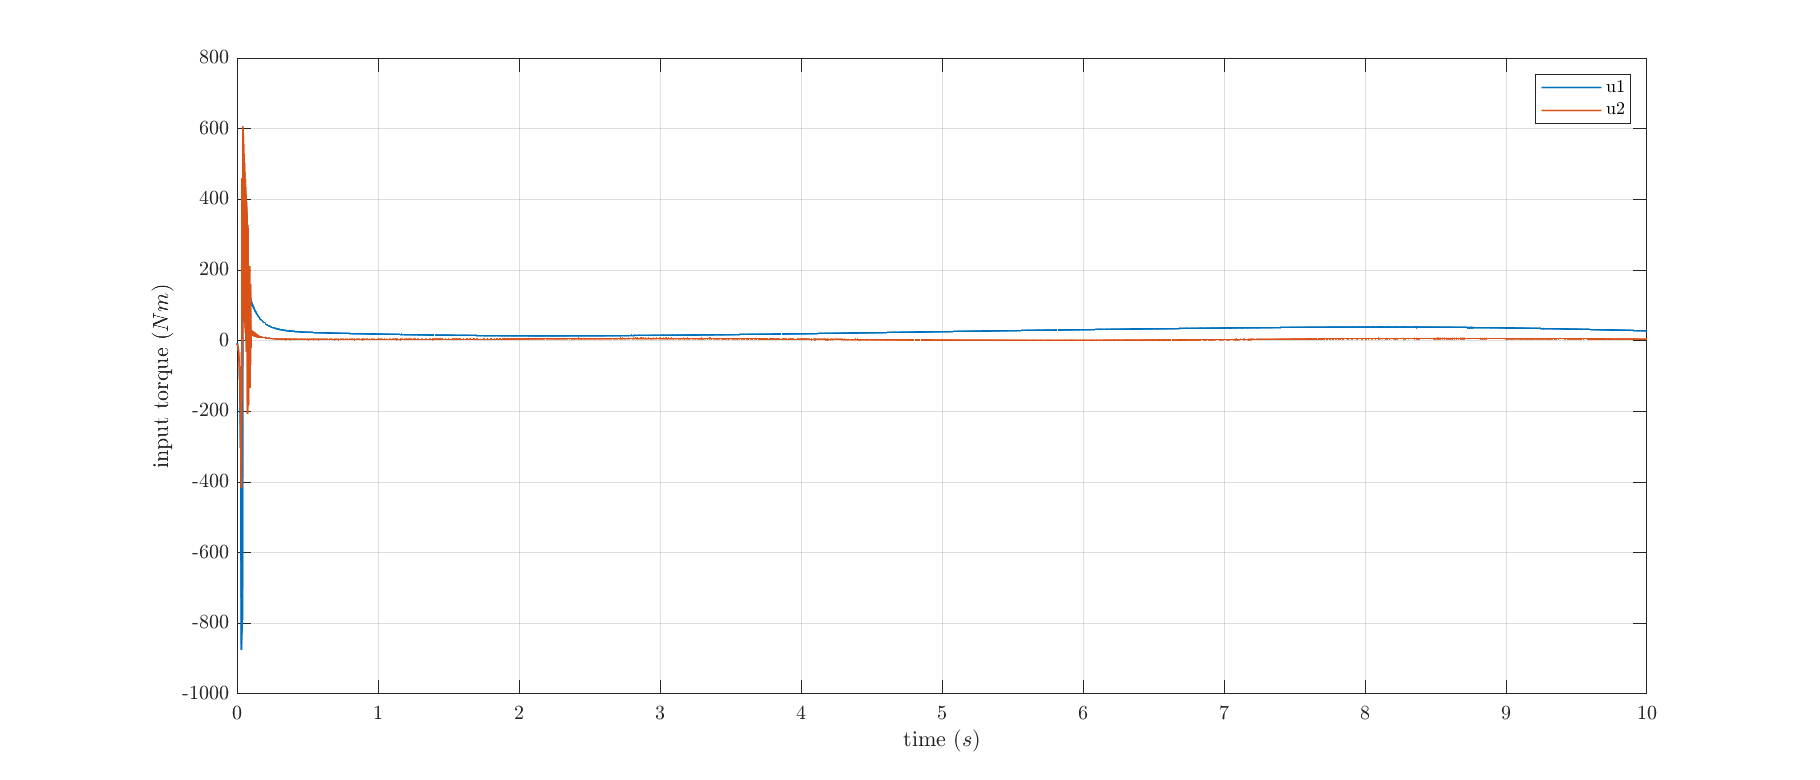
\includegraphics[width=15cm]{fig/sim2/lincrease/ulincrease.png}
    \caption{Control input with respect to time for $\lambda_1=10$ and $\lambda_2=20$}
\end{figure}
\begin{figure}[H]
    \centering
    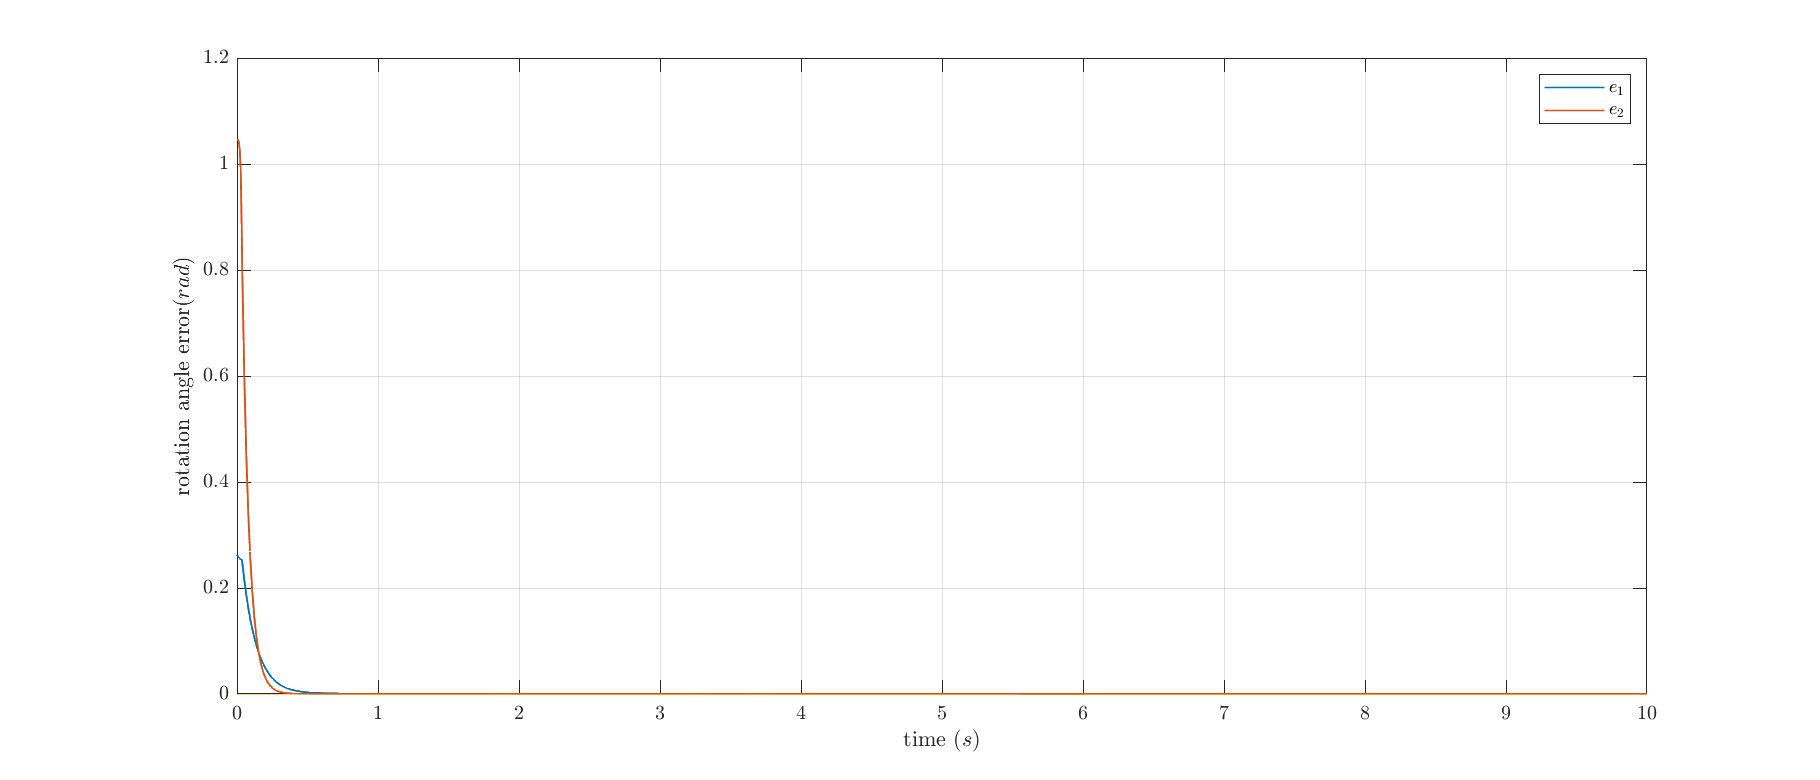
\includegraphics[width=15cm]{fig/sim2/lincrease/elincrease.png}
    \caption{State error with respect to time for $\lambda_1=10$ and $\lambda_2=20$}
\end{figure}

\noindent\hspace{-2pt}
Comparing figures 18 and 35, we can see that for decreased $\lambda_1$ and $\lambda_2$ values, the convergence to the 
desired state curve is delayed noticeably, as expected. Reduced $\lambda$ values lead to reduced convergence speed, since 
the system reaches $s=0$ surface. The corresponding state error reduces slower too (figures 28 and 36). On the other hand, 
when we increase $\lambda$ values, we notice faster convergence (comparing figures 18 and 28 with 37 and 39 respectively). 
However, the improvement does not look satisfying and at the same time, the control input (figure 38) presents a much larger maximum 
amplitude than the case with the selected parameters (figure 23) and that should be avoided. For that reason, we avoid increasing 
$\lambda$ values.

\end{document}

